\documentclass[11pt,a4paper,twoside]{scrreprt}
\KOMAoptions{cleardoublepage=empty}

% ---------- Base encoding & fonts ----------
\usepackage[T1]{fontenc}
\usepackage[utf8]{inputenc}
\usepackage{lmodern}
\usepackage{microtype}
\usepackage{accsupp}  % lets us control ActualText for copy/paste

\DeclareRobustCommand{\copyspace}{%
  \BeginAccSupp{ActualText= }%  % what the clipboard receives (a real U+0020)
  \kern0pt\ %                    % what is drawn (a normal space)
  \EndAccSupp
}
% ---------- Graphics & links ----------
\usepackage{graphicx}
\usepackage[dvipsnames]{xcolor}
\usepackage{hyperref}
\hypersetup{
  colorlinks=true,
  linkcolor=blue!60!black,
  urlcolor=blue!60!black,
  citecolor=blue!60!black
}

% ---------- Lists, tables, floats ----------
\usepackage{enumitem}                % for [nosep]
\usepackage{booktabs}                % \toprule etc.
\usepackage{float}                   % [H] placement
\usepackage{tabularx,array}
\renewcommand{\arraystretch}{1.15}

% ---------- KOMA (safe if class is scrreprt/scrartcl) ----------
\makeatletter
\@ifundefined{KOMAClassName}{}{%
  \KOMAoptions{
    DIV=14,
    BCOR=0mm,
    headinclude=true,
    footinclude=false
  }%
}
\makeatother

% ---------- Numbering & ToC ----------
\setcounter{secnumdepth}{3}
\setcounter{tocdepth}{3}             % show down to subsubsection in ToC
\renewcommand\thesection{\arabic{section}}
\renewcommand\thesubsection{\thesection.\arabic{subsection}}
\renewcommand\thesubsubsection{\thesubsection.\arabic{subsubsection}}

% ---------- Small helpers ----------
\newcommand{\keil}{\textbf{Keil uVision5}}
\providecommand{\tightlist}{\setlength{\itemsep}{0pt}\setlength{\parskip}{0pt}}

% ---------- Listings: ARM assembly (colors + top/bottom rules only) ----------
\usepackage{listings}
\usepackage{listingsutf8}

% Palette
\definecolor{AsmMnemonic}{HTML}{005CC5}   % blue
\definecolor{AsmDirective}{HTML}{6F42C1}  % purple
\definecolor{AsmCond}{HTML}{D73A49}       % red
\definecolor{AsmRegister}{HTML}{22863A}   % green
\definecolor{AsmComment}{HTML}{6A737D}    % gray
\definecolor{AsmLineNo}{HTML}{9AA0A6}     % light gray
\definecolor{AsmRule}{HTML}{C0C4C8}       % rule color

% Language
\lstdefinelanguage{Assembler}{
  % Mnemonics (include S-suffixed forms and conditional branch forms)
  morekeywords={
    ADC,ADCS,ADD,ADDS,ADR,AND,ANDS,ASR,ASRS,
    B,BEQ,BNE,BCS,BHS,BCC,BLO,BMI,BPL,BVS,BVC,BHI,BLS,BGE,BLT,BGT,BLE,BAL,
    BL,BLX,BX,
    CBNZ,CBZ,CLZ,CMP,CMN,
    EOR,EORS,
    ISB,
    LDM,LDR,LDRB,LDRH,
    LSL,LSLS,LSR,LSRS,
    MOV,MOVS,MOVT,MOVW,MSR,MRS,
    MUL,MULS,
    NOP,
    ORR,ORRS,
    POP,PUSH,
    REV,REV16,REVSH,
    ROR,RORS,
    SBC,SBCS,
    SEV,
    STM,STR,STRB,STRH,
    SUB,SUBS,
    TBB,TBH,TST,
    UXTB,UXTH,UXTB16,
    WFE,WFI,
    YIELD,
    BKPT
  },
  % Directives
  morekeywords=[2]{AREA,ALIGN,DCD,DCB,DCW,EXPORT,IMPORT,ENTRY,END,SPACE,KEEP,WEAK,LTORG,PROC,ENDP},
  % Condition-code tokens (when written separately; kept for completeness)
  morekeywords=[3]{EQ,NE,CS,HS,CC,LO,MI,PL,VS,VC,HI,LS,GE,LT,GT,LE,AL},
  morecomment=[l]{;},
  sensitive=true
}
\lstdefinelanguage[ARM]{Assembler}[]{Assembler}{}


\lstdefinestyle{labcode}{
  language={[ARM]Assembler},
  inputencoding=utf8,
  basicstyle=\ttfamily\small,  % inconsolata will be used
  columns=fixed,               % fixed-width columns -> real spaces in PDF
  keepspaces=true,             % preserve all spaces (incl. leading)
  tabsize=4,                   % set to the width you expect; or convert tabs to spaces
  showstringspaces=false,
  upquote=true,
  keywordstyle={\color{AsmMnemonic}\bfseries},
  keywordstyle=[2]{\color{AsmDirective}\bfseries},
  keywordstyle=[3]{\color{AsmCond}\bfseries},
  commentstyle={\itshape\color{AsmComment}},
  emph={R0,R1,R2,R3,R4,R5,R6,R7,R8,R9,R10,R11,R12,SP,LR,PC,
        APSR,IP,PSP,MSP,xPSR},
  emphstyle={\color{AsmRegister}\bfseries},
  showstringspaces=false,
  tabsize=2,
  keepspaces=true,
  columns=fullflexible,
  % line breaking
  breaklines=true,
  breakatwhitespace=true,
  % frame: top & bottom only
  frame=lines,
  rulecolor={\color{AsmRule}},
  xleftmargin=2em,
  framexleftmargin=2em,
  % line numbers
  % line numbers disabled
  % float control
  float,
  floatplacement=H,
  captionpos=b,
}
\lstset{style=labcode}
\usepackage{amsmath}
\usepackage{tcolorbox}
\usepackage{tikz}
\usetikzlibrary{positioning,arrows.meta,decorations.pathreplacing}
\usepackage{subcaption} % or subfig if you prefer
% ---------- Chapter-level ToCs ----------

% ---------- Tables of contents ----------
\usepackage{etoc}  % local ToCs that inherit the same style as \tableofcontents
\usepackage{titletoc}  % for \titlecontents command
% ---------- Cover page config ----------
% If you use an SVG logo, keep this. If you prefer PNG/PDF, you may omit.
\usepackage{svg} % requires --shell-escape or inkscape; else convert logo to PDF/PNG

% Editable cover fields

% ---- Technical manual title page helpers ----
% Logo is expected at assets/<name>.svg; adjust if needed.
\svgpath{{resources/}} % where the logo lives

\providecommand{\LOGONAME}{birzeit-logo} % base name, no extension
\providecommand{\DEPARTMENT}{Department of Electrical \& Computer Engineering}
\providecommand{\COURSENUM}{ENCS4110}
\providecommand{\COURSENAME}{Computer Design Laboratory}
% ---- Cover defaults (override as needed) ----
\providecommand{\ManualSubtitle}{Laboratory Manual}

% Semantic version pieces (or set \ManualVersion directly)
\providecommand{\ManualVersionMajor}{1}
\providecommand{\ManualVersionMinor}{0}
\providecommand{\ManualVersionPatch}{0}
\providecommand{\ManualVersion}{v\ManualVersionMajor.\ManualVersionMinor.\ManualVersionPatch}
\newcommand{\MonthYear}{%
  \ifcase\month
  \or January\or February\or March\or April\or May\or June%
  \or July\or August\or September\or October\or November\or December
  \fi~\the\year
}
% Local ToC etc. can stay as-is. Ensure svg path is set:
\makeatletter
\newcommand{\maketechnicaltitlepage}{%
  \begin{titlepage}
    \thispagestyle{empty}

    % --- Top: logo + department + course ---
    \vspace*{1.2cm}
    \begin{center}
      \IfFileExists{assets/\LOGONAME.pdf}
        {\includegraphics[width=.80\textwidth]{assets/\LOGONAME.pdf}}
        {\includesvg[width=.80\textwidth,inkscapelatex=false]{\LOGONAME}}

      \vspace{0.3cm}
      {\large \DEPARTMENT\par}
      {\large \COURSENUM\;--\;\COURSENAME\par}
    \end{center}

    % --- Middle: centered Title + Subtitle ONLY ---
    \vspace{1.5cm}
    \begin{center}
      {\Huge\bfseries \@title\par}
      \vspace{0.35cm}
      {\Large \ManualSubtitle\par}
    \end{center}
    \vfill

    % --- Bottom-left: Version + Date ---
    \begin{flushleft}
      {\large \textbf{Version:} \ManualVersion}\\[0.2cm]
        {\large \textbf{Date:} \MonthYear}
    \end{flushleft}
  \end{titlepage}%
}
\makeatother

% ---- titletoc formatting: Tufte-ish, robust ----
\usepackage{titletoc}

\titlecontents{part}%
  [0pt]% distance from left margin
  {\addvspace{0.25\baselineskip}}% above (global formatting of entry)
  {\allcaps{Part~\thecontentslabel}\quad}% before w/ label (label = ``Part I'')
  {\allcaps{Part~\thecontentslabel}\allcaps}% before w/o label
  {}% filler and page (leaders and page num)
  [\vspace*{0.5\baselineskip}]% after

\titlecontents{chapter}%
    [4em]% distance from left margin
    {}% above (global formatting of entry)
    {\contentslabel{2em}\textit}% before w/ label (label = ``Chapter 1'')
    {\hspace{0em}\textit}% before w/o label
    {\qquad\thecontentspage}% filler and page (leaders and page num)
    [\vspace*{0.5\baselineskip}]% after
%%%% End additional code by Kevin Godby


% Silent part: adds a numbered Part entry to the ToC, prints nothing
% --- ToC-only “Part” entry (no heading printed, no hyperlink in ToC) ---
\makeatletter
\newcommand{\toconlypart}[1]{%
  \clearpage                 % keep if you want a clean break; remove if not
  \refstepcounter{part}%     % step the Part counter (I, II, …)
  % Write a plain (non-hyperlinked) contents line: 4th arg = link target -> empty
  \addtocontents{toc}{%
    \protect\contentsline{part}{\protect\numberline{\thepart}#1}{\thepage}{}%
  }%
  % Optional: set header marks if you use \leftmark/\rightmark
  \markboth{Part \thepart\quad #1}{}%
}
\makeatother


\usepackage{bytefield}
\usepackage[table]{xcolor} % for light gray shading
\usepackage{needspace}


\usepackage{graphicx} % for \resizebox
\usepackage{calc}     % for \widthof
\usepackage{bytefield}

% measure once
\newlength{\pfbit}
\settowidth{\pfbit}{\tiny PF0} % or {\scriptsize PF0} if you prefer

\providecommand{\allcaps}[1]{\MakeUppercase{#1}}




\providecommand{\LOGONAME}{birzeit-logo} % base name, no extension
\providecommand{\DEPARTMENT}{Department of Electrical \& Computer Engineering}
\providecommand{\COURSENUM}{ENCS4110}
\providecommand{\COURSENAME}{Computer Design Laboratory}
\title{Laboratory Manual}
\renewcommand{\ManualSubtitle}{TM4C123 LaunchPad (ARM Cortex-M4)}
\renewcommand{\ManualVersionMajor}{1}
\renewcommand{\ManualVersionMinor}{0}
\renewcommand{\ManualVersionPatch}{0}

\date{\today}

\begin{document}

\maketechnicaltitlepage
% Global ToC: all experiments with main sections
\cleardoublepage
\begingroup
\setcounter{tocdepth}{3} % show chapters and sections only
\tableofcontents
\endgroup
\cleardoublepage

\toconlypart{ARM Assembly Language Programming}
\chapter{ARM Cortex-M4 Assembly Fundamentals}

\section*{Learning Objectives}
\begin{itemize}[nosep]
  \item Describe the Cortex-M4 register set, xPSR flags, and ARMv7-M memory map.
  \item Write and assemble a minimal ARM program with a vector table and \texttt{Reset\_Handler}.
  \item Use core data-processing, shift/rotate, and compare/test instructions.
  \item Apply conditional execution with condition codes (e.g., \texttt{ADDEQ}, \texttt{BNE}).
  \item Debug in \keil: set breakpoints, single-step, inspect registers/memory, and interpret flags.
\end{itemize}

\section*{Experiment Overview}
This experiment introduces low-level programming on the Cortex-M4. You will build a minimal startup image, practice common data-processing and control-flow instructions, and use the \keil\ debugger to observe register and memory effects while stepping through code. By the end, you will be able to implement and test short assembly routines that manipulate data and make decisions based on condition flags.

\newpage
\tableofcontents
\newpage
\section{Theoretical Background}
\subsection{Cortex-M4 Architecture}
\subsubsection{Registers Overview}
The Cortex-M4 architecture includes a set of general-purpose registers (R0-R12), a stack pointer (SP), a link register (LR), a program counter (PC), and a program status register (xPSR), all of which are 32-bit registers. The general-purpose registers are used for data manipulation and temporary storage during program execution. The SP is used to manage the call stack, while the LR holds the return address for function calls. The PC points to the next instruction to be executed, and the xPSR contains flags and status information about the processor state.
\paragraph{Program Status Register (xPSR)}
holds the current state of the processor, including condition flags (Negative, Zero, Carry, Overflow), interrupt status, and execution state. These flags are updated based on the results of arithmetic and logical operations, allowing for conditional branching and decision-making in programs.

\subsubsection{Memory Mapping}
The Cortex-M4 uses a flat memory model, where all memory locations are accessible through a single address space. This model simplifies programming and allows for efficient access to data and instructions. The memory is divided into several regions, including code memory (for storing instructions), data memory (for storing variables), and peripheral memory (for interfacing with hardware components). The architecture supports both little-endian and big-endian data formats, with little-endian being the default.
\begin{table}[H]
\centering
\caption{Cortex-M4 Memory Regions (ARMv7-M)}
\begin{tabularx}{\linewidth}{@{}p{0.20\linewidth}p{0.30\linewidth}X@{}}
\toprule
\textbf{Region} & \textbf{Address Range} & \textbf{Description} \\
\midrule
Code            & \texttt{0x00000000}--\texttt{0x1FFFFFFF} & Flash memory for program code \\[0.5ex]
SRAM            & \texttt{0x20000000}--\texttt{0x3FFFFFFF} & On-chip static RAM for data \\[0.5ex]
Peripheral      & \texttt{0x40000000}--\texttt{0x5FFFFFFF} & Memory-mapped peripheral registers \\[0.5ex]
External RAM    & \texttt{0x60000000}--\texttt{0x9FFFFFFF} & External RAM (if implemented) \\[0.5ex]
External Device & \texttt{0xA0000000}--\texttt{0xDFFFFFFF} & External devices/memory (if implemented) \\[0.5ex]
Private Peripheral Bus & \texttt{0xE0000000}--\texttt{0xE00FFFFF} & Cortex-M4 internal peripherals  (NVIC, SysTick, MPU, SCB)\\
System          & \texttt{0xE0100000}--\texttt{0xFFFFFFFF} & System region (reserved/system-level) \\
\bottomrule
\end{tabularx}
\end{table}


\subsection{Assembly Language Basics}

Assembly language is a low-level programming language that provides a direct correspondence between human-readable instructions and the machine code executed by the processor. Each instruction encodes a specific operation, such as moving data, performing arithmetic or logic, or altering control flow. Because it maps so closely to hardware, assembly allows precise control of system resources and is commonly used in performance-critical routines or when direct access to hardware is required.

Assembly programs are typically composed of three main elements: \emph{instructions}, \emph{directives}, and \emph{labels}.

\paragraph{Instructions}  
Instructions are the executable commands that the CPU carries out. Examples include data movement (\texttt{MOV}), arithmetic (\texttt{ADD}, \texttt{SUB}), logical operations (\texttt{AND}, \texttt{ORR}), and control flow (\texttt{B}, \texttt{BL}). Each instruction directly translates to one or more machine code opcodes and determines the actual behavior of the program.

\paragraph{Directives}  
Directives are commands to the assembler that guide how source code is translated into machine code but do not generate instructions themselves. Common examples include \texttt{AREA} (define a code or data section), \texttt{ALIGN} (align data to memory boundaries), \texttt{DCD} (allocate and initialize a word of storage), and \texttt{EXPORT} (export a symbol for linking). Directives organize program layout, control memory allocation, and manage symbol visibility.

\paragraph{Labels}  
Labels are symbolic names that mark specific locations in code or data. They act as targets for jumps and branches or as references for data access. Labels improve program readability and maintainability by avoiding hard-coded addresses. For instance, a label like \texttt{loop\_start} can be used as the destination of a branch instruction, and the assembler automatically computes the correct relative address.
\subsubsection{Instruction Set Overview}
The ARM Cortex-M4 instruction set is a subset of the ARMv7-M architecture, designed for efficient execution in embedded systems. It includes a variety of instructions for data processing, memory access, and control flow. Key categories of instructions include:
\hfill
\begin{itemize}[nosep]
    \item \textbf{Data Processing Instructions}: These include arithmetic operations (e.g., \texttt{ADD}, \texttt{SUB}), logical operations (e.g., \texttt{AND}, \texttt{ORR}), and data movement instructions (e.g., \texttt{MOV}, \texttt{MVN}).
    \item \textbf{Load and Store Instructions}: Instructions like \texttt{LDR} (load register) and \texttt{STR} (store register) are used to transfer data between registers and memory.
    \item \textbf{Branch Instructions}: Control flow is managed using branch instructions such as \texttt{B} (branch), \texttt{BL} (branch with link), and conditional branches like \texttt{BEQ} (branch if equal).
    \item \textbf{Special Instructions}: These include instructions for system control, such as \texttt{NOP} (no operation), \texttt{WFI} (wait for interrupt), and instructions for manipulating the stack and handling exceptions.
\end{itemize}
\subsubsection{General Instruction Format}

Assembly source lines generally follow this shape:

\[
\texttt{[label]} \quad \texttt{OPCODE\{<cond>\}\{S\}} \quad \texttt{operands} \quad \texttt{\color{lightgray}; comment}
\]

where curly braces \texttt{\{\}} denote optional components, and:
\begin{itemize}[nosep]
  \item \texttt{label}: optional symbolic name marking the current address.
  \item \texttt{OPCODE}: instruction mnemonic (e.g., \texttt{ADD}, \texttt{MOV}, \texttt{B}).
  \item \texttt{<cond>}: optional condition code (e.g., \texttt{EQ}, \texttt{NE}, \texttt{LT}, \texttt{GE}) that predicates execution.
  \item \texttt{S}: optional suffix indicating whether to update the condition flags (e.g., \texttt{ADDS}).
  \item \texttt{operands}: registers, immediates, or memory operands (e.g., \texttt{R0, R1, \#1} or \texttt{[R2]}).
  \item Anything after a semicolon (\texttt{;}) is a comment ignored by the assembler.
\end{itemize}

\begin{lstlisting}[caption={Instruction format example}]
loop_start   ADDS   R0, R0, #1      ; R0 = R0 + 1, update flags (N,Z,C,V)
             CMP    R0, #10         ; compare R0 with 10 (sets flags)
             BLT    loop_start      ; branch if R0 < 10 (uses flags)
\end{lstlisting}
\subsubsection{Conditional Execution}

Most ARM instructions can be made \emph{conditional} by appending a two-letter
\emph{condition code} to the mnemonic (e.g., \texttt{ADDEQ}, \texttt{ADDNE}).
The instruction is executed only if the condition evaluates true based on the
\texttt{xPSR} flags $N$ (negative), $Z$ (zero), $C$ (carry), and $V$ (overflow).
When no condition is supplied, the default is \texttt{AL} (always).

\begin{table}[H]
\centering
\caption{Common ARM Condition Codes}
\small
\begin{tabularx}{0.72\linewidth}{@{}l l X@{}}
\toprule
\textbf{Cond.} & \textbf{Meaning} & \textbf{Description} \\
\midrule
EQ  & Equal                     & Execute if $Z=1$. \\
NE  & Not equal                 & Execute if $Z=0$. \\
CS/HS & Carry set / Unsigned higher or same & Execute if $C=1$. \\
CC/LO & Carry clear / Unsigned lower        & Execute if $C=0$. \\
MI  & Minus (negative)          & Execute if $N=1$. \\
PL  & Plus (non-negative)       & Execute if $N=0$. \\
VS  & Overflow set              & Execute if $V=1$. \\
VC  & Overflow clear            & Execute if $V=0$. \\
HI  & Unsigned higher           & Execute if $C=1$ \emph{and} $Z=0$. \\
LS  & Unsigned lower or same    & Execute if $C=0$ \emph{or} $Z=1$. \\
GE  & Greater or equal (signed) & Execute if $N=V$. \\
LT  & Less than (signed)        & Execute if $N\neq V$. \\
GT  & Greater than (signed)     & Execute if $Z=0$ \emph{and} $N=V$. \\
LE  & Less or equal (signed)    & Execute if $Z=1$ \emph{or} $N\neq V$. \\
AL  & Always                    & Always execute (default if no condition). \\
NV  & Never                     & Reserved / do not use. \\
\bottomrule
\end{tabularx}
\end{table}

\noindent\textit{Example:}
\begin{lstlisting}[caption={Using conditional-suffix mnemonics},label={lst:cond-exec}]
        CMP     R0, #0          ; set flags from (R0 - 0)
        ADDEQ   R1, R1, #1      ; if Z==1: R1++
        ADDNE   R2, R2, #1      ; if Z==0: R2++
\end{lstlisting}

\subsubsection{Barrel Shifter}
    
The barrel shifter is a hardware feature that allows …is a hardware feature that allows for efficient shifting and rotating of register values as part of data processing instructions. It can perform operations such as logical shifts (left or right), arithmetic shifts, and rotations on the second operand (\texttt{Operand2}) before it is used in the instruction without wasting extra instructions or cycles.

\noindent Examples of barrel shifter usage:
\begin{lstlisting}[caption={Barrel shifter examples}]
    ADD    R0, R2, R1, LSL #2    ; R0 = R2 + (R1 << 2) using barrel shifter
    SUB    R3, R4, R5, LSR #1    ; R3 = R4 - (R5 >> 1) using barrel shifter
    ORR    R6, R7, R8, ROR #3    ; R6 = R7 | (R8 rotated right by 3)
\end{lstlisting}

\newpage
\subsection{Basic Program Template (Boilerplate)}

The minimal skeleton below shows a valid vector table in a \texttt{READONLY} \texttt{RESET} area, a \texttt{READWRITE} data area for variables, and a code area with the \texttt{Reset\_Handler} entry point.

\begin{lstlisting}[caption={Cortex-M4 boilerplate with READWRITE data}]
        AREA    RESET, CODE, READONLY     ; Vector table lives in read-only code
        EXPORT  __Vectors                 ; Make symbol visible to the linker
__Vectors
        DCD     0x20001000                ; Initial SP value (top of stack in SRAM)
        DCD     Reset_Handler             ; Reset vector: entry address
        ALIGN        
        ; -------------------- Read-Write Data --------------------
        AREA    M_DATA, DATA, READWRITE   ; Variables go here (RAM)
        EXPORT  COUNT                     ; Export if referenced by other modules
COUNT   DCD     0                         ; Initialized RW variable (word)
BUF     SPACE   16                        ; Uninitialized RW buffer (16 bytes)
        ALIGN        
        ; -------------------- Application Code -------------------
        AREA    MYCODE, CODE, READONLY
        ENTRY
        EXPORT  Reset_Handler
Reset_Handler
        ; Example: COUNT++ and store to BUF[0]
        LDR     R0, =COUNT                ; R0 <- &COUNT
        LDR     R1, [R0]                  ; R1 <- COUNT
        ADDS    R1, R1, #1                ; R1 = R1 + 1 (update flags)
        STR     R1, [R0]                  ; COUNT <- R1        
        LDR     R2, =BUF                  ; R2 <- &BUF
        STRB    R1, [R2]                  ; BUF[0] <- (low byte of R1)
STOP    B       STOP                      ; Stay here forever
        END
\end{lstlisting}

\paragraph{What each directive does}
\begin{itemize}[nosep]
  \item \texttt{AREA <name>, CODE|DATA, READONLY|READWRITE}:
        defines a section. Put the vector table and program text in \texttt{CODE, READONLY};
        put variables in \texttt{DATA, READWRITE}.
  \item \texttt{EXPORT <symbol>}: makes a label visible to the linker/other modules.
  \item \texttt{DCD, DCW, DCB <values>}: allocate and initialize words, halfwords, or bytes.
  \item \texttt{SPACE <n>}: reserve \textit{n} bytes of uninitialized storage in RAM.
  \item \texttt{ALIGN}: align to a suitable boundary (commonly 4 bytes for words).
  \item \texttt{ENTRY}: mark the entry point of the image for the toolchain.
  \item \texttt{END}: end of source file.
\end{itemize}

\paragraph{Notes}
\begin{itemize}[nosep]
    \item The first two words in \texttt{\_\_Vectors} must be the initial stack pointer value and the address of \texttt{Reset\_Handler}.
    \item The assembler/linker places sections in appropriate memory regions based on the target device and linker script.
    \item Labels must start at the beginning of the line (no indentation), while instructions and directives should be indented for proper assembly.
    \item Variables in \texttt{READWRITE} areas are initialized to zero by default. While you can specify initial values using directives like \texttt{DCD}, the linker will place these in flash and copy them to RAM during startup, or they may be zeroed out during RAM initialization.
\end{itemize}

\newpage
\section{Procedure}
\subsection{Setting Up the Keil uVision5 Environment}
Make sure you have the \keil\ IDE installed on your computer. If not, download and install it from the official Keil website (\url{https://www.keil.com/demo/eval/arm.htm}).
\subsubsection{Creating a New Project}
\begin{enumerate}[nosep]
    \item Open \keil\ and create a new project:
    \begin{itemize}[nosep]
        \item Go to \texttt{Project > New uVision Project...}
        \item Choose a directory and name for your project (e.g., \texttt{Exp01\_ARM\_Assembly}).
    \end{itemize}
    \item Select the target device:
    \begin{itemize}[nosep]
        \item In the "Select Device for Target" dialog, choose ARM Cortex-M4 (ARMCM4) as we will be using it only for simulation.
        \item Click "OK" to confirm.
    \end{itemize}
    \item Configure project settings:
    \begin{itemize}[nosep]
        \item Go to \texttt{Project > Options for Target 'Target 1'...}
        \item Under the "Debug" tab, select "Use Simulator" as the debug driver.
    \end{itemize}
    \item Add a new assembly file to the project:
    \begin{itemize}[nosep]
        \item Right-click on "Source Group 1" in the Project window and select \texttt{Add New Item to Group 'Source Group 1'...}
        \item In the "Add New Item" dialog, select "Assembly File" from the list.
        \item Name the file (e.g., \texttt{main.s}) and click "Add".
    \end{itemize}
    \item Build the project:
    \begin{itemize}[nosep]
        \item Click on the "Build" button (or go to \texttt{Project > Build Target}), or use the shortcut \texttt{F7}.
        \item Check the "Output" window for any errors or warnings. If there are errors, fix them in your assembly code and rebuild.
        \item Once the build is successful, you should see a message indicating that the build was completed without errors.
    \end{itemize}
    \item Start a debugging session:
    \item Click on the "Debug" button (or go to \texttt{Debug > Start/Stop Debug Session}), or use the shortcut \texttt{Ctrl + F5}.
\end{enumerate}
\subsubsection{Debugging and Running the Program}
\begin{figure}[H]
    \centering
    \includegraphics[width=\textwidth]{resources/keil_debug.png}
    \caption{Keil uVision5 Debugging Interface}
    \label{fig:keil_debug}
\end{figure}
Figure \ref{fig:keil_debug} shows the Keil uVision5 debugging interface. You can run and debug your assembly program using two main approaches:
\begin{enumerate}[nosep]
    \item \textbf{Step by Step Execution}:
    \begin{itemize}[nosep]
        \item Use the "Step" button (or press \texttt{F11}) marked in green in Figure \ref{fig:keil_debug} to execute your program one instruction at a time.
        \item Observe the changes in the registers and memory as you step through each instruction.
    \end{itemize}
    \item \textbf{Run the entire program}:
    \begin{itemize}[nosep]
        \item Use the "Run" button (or press \texttt{F5}) marked in blue in Figure \ref{fig:keil_debug} to execute your program continuously until it hits a breakpoint or completes execution.
        \item After running, you must stop the execution using the "Stop" button marked in yellow in Figure \ref{fig:keil_debug}.
        \item Check the final values in the registers and memory to verify the program's behavior.
    \end{itemize}
\end{enumerate}
\newpage
\subsection{Examples}
\subsubsection{Example 1: Simple Arithmetic Operations and Flag Manipulation}
The following example demonstrates basic arithmetic operations, flag manipulation, and conditional execution using ARM assembly language. It includes comments to guide you through each step.
\lstinputlisting[caption={Example 1: Simple Arithmetic Operations and Flag Manipulation}]{snippets/assembly/exp1/example1.asm}
\newpage
\subsubsection{Example 2: Using the Barrel Shifter and Conditional Execution}
The following example demonstrates the use of the barrel shifter for efficient data manipulation and conditional execution based on status flags. It includes comments to guide you through each step.
\lstinputlisting[caption={Example 2: Using the Barrel Shifter and Conditional Execution}]{snippets/assembly/exp1/example2.asm}


\chapter{ARM Cortex-M4 Instructions and Addressing Modes}
\section*{Learning Objectives}
After completing this experiment, you will be able to:
\begin{itemize}[nosep]
  \item Classify ARM Cortex-M4 instructions into data-processing, load/store, and branch categories.
  \item Perform arithmetic, logical, and shift/rotate operations using data-processing instructions (including \texttt{Operand2} with the barrel shifter).
  \item Move data between registers and memory using load/store instructions with immediate, register-offset, and pre-/post-indexed addressing modes.
  \item Declare and initialize data objects (arrays, strings, buffers) with assembler directives, and use pointers to access and modify them.
  \item Trace how instructions affect registers and xPSR flags using the \keil\ debugger (breakpoints, single-step, register/memory views).
\end{itemize}
\section*{Experiment Overview}
This experiment develops fluency with the ARM Cortex-M4 instruction set for data manipulation and memory access. 
You will practice using arithmetic, logical, and shift/rotate instructions, and learn how data moves between registers and memory through load/store instructions and their addressing modes. 
You will also define data with assembler directives and use pointers to read and update memory.

\noindent In this experiment, you will:
\begin{itemize}[nosep]
  \item Write and run short assembly routines that use data-processing instructions to transform register values.
  \item Apply immediate, register-offset, and pre-/post-indexed addressing modes to load from and store to memory.
  \item Define arrays, strings, and buffers with directives, and use pointers to traverse and modify them.
  \item Observe instruction effects on registers and flags with the \keil\ debugger to verify correctness.
\end{itemize}

By the end of this lab, you will be able to implement, assemble, and debug Cortex-M4 programs that perform register-level computation and structured memory access—providing the foundation for flow control and procedure calls in later experiments.

\newpage
\etocsetnexttocdepth{subsubsection}
\localtableofcontents
\bigskip
\newpage
\section{Theoretical Background}
As mentioned in Experiment 1, assembly instructions are split into three main categories: data processing, load/store, and branch instructions. This experiment focuses on data processing instructions, load/store instructions and their addressing modes. branch instructions and flow control will be covered in the next experiment.
\subsection{Data Processing Instructions}
Data processing instructions perform arithmetic and logical operations on data stored in registers. They can also manipulate the condition flags in the xPSR based on the results of the operations. Common data processing instructions take the following form:
\[
\begin{aligned}
\texttt{\{LABEL\}} \quad & \texttt{OPCODE\{<cond>\}\{S\} Rd, Rn, Operand2}
\end{aligned}
\]

where:
\begin{itemize}[nosep]
    \item \texttt{LABEL}: optional label for branching.
    \item \texttt{OPCODE}: the operation to be performed (e.g., \texttt{ADD}, \texttt{SUB}, \texttt{AND}, \texttt{ORR}).
    \item \texttt{<cond>}: optional condition code that predicates execution.
    \item \texttt{S}: optional suffix indicating whether to update the condition flags.
    \item \texttt{Rd}: destination register where the result is stored.
    \item \texttt{Rn}: first operand register.
    \item \texttt{Operand2}: second operand, which can be an immediate value limited to 8 bits, a register, or a barrel shifter operation (see Section~\ref{sec:barrel-shifter}).
\end{itemize}


\subsubsection{Arithmetic Instructions}
Arithmetic instructions perform basic mathematical operations. Some common arithmetic instructions include addition, subtraction, multiplication, and their variants. The following table summarizes some of the most commonly used arithmetic instructions in the ARM Cortex-M4 architecture.
\begin{table}[H]
\centering
\caption{Common ARM Cortex-M4 Arithmetic Instructions}
\small
\begin{tabularx}{\linewidth}{@{}l l l X@{}}
\toprule
\textbf{Instr.} & \textbf{Syntax} & \textbf{Operation} & \textbf{Description} \\
\midrule
ADD  & \texttt{ADD\{S\} Rd, Rn, Operand2}
     & $Rd \leftarrow Rn + Operand2$
     & \emph{Operand2} may be a register, an immediate, or a shifted register. \\
ADC  & \texttt{ADC\{S\} Rd, Rn, Operand2}
     & $Rd \leftarrow Rn + Operand2 + C$
     & Adds carry-in $C$. \\
SUB  & \texttt{SUB\{S\} Rd, Rn, Operand2}
     & $Rd \leftarrow Rn - Operand2$
     & Standard subtraction. \\
SBC  & \texttt{SBC\{S\} Rd, Rn, Operand2}
    & $Rd \leftarrow Rn - Operand2 - \overline{C}$
    & Subtract with carry. If carry flag is clear, result is reduced by one. Used for multiword arithmetic. \\
RSB  & \texttt{RSB\{S\} Rd, Rn, Operand2}
     & $Rd \leftarrow Operand2 - Rn$
     & Reverse subtract. \\
MUL  & \texttt{MUL\{S\} Rd, Rn, Rm}
     & $Rd \leftarrow (Rn \times Rm)_{[31{:}0]}$
     & 32$\times$32 $\rightarrow$ low 32 bits. \\
MLA  & \texttt{MLA Rd, Rn, Rm, Ra}
     & $Rd \leftarrow (Rn \times Rm) + Ra$
     & Multiply-accumulate. \\
MLS  & \texttt{MLS Rd, Rn, Rm, Ra}
     & $Rd \leftarrow Ra - (Rn \times Rm)$
     & Multiply-subtract. \\
UMULL & \texttt{UMULL RdLo, RdHi, Rn, Rm}
      & $\{RdHi,RdLo\} \leftarrow Rn \times Rm$
      & Unsigned 32$\times$32 $\rightarrow$ 64-bit product. \\
SMULL & \texttt{SMULL RdLo, RdHi, Rn, Rm}
      & $\{RdHi,RdLo\} \leftarrow Rn \times Rm$
      & Signed 32$\times$32 $\rightarrow$ 64-bit product. \\
\bottomrule
\end{tabularx}

\vspace{2pt}
\footnotesize\emph{Note:} $C$ denotes the carry flag in \texttt{xPSR}. \emph{Operand2} may be an immediate or a shifted register depending on the encoding.
\end{table} 
\subsubsection{Logical and Move Instructions}
Logical instructions perform bitwise operations on data, while move instructions transfer data between registers or load immediate values. The following table summarizes some of the most commonly used logical and move instructions in the ARM Cortex-M4 architecture.
\begin{table}[H]
\centering
\caption{Logical and Move Instructions}
\small
\begin{tabularx}{\linewidth}{@{}l l l X@{}}
\toprule
\textbf{Instr.} & \textbf{Syntax} & \textbf{Operation} & \textbf{Description} \\
\midrule
AND  & \texttt{AND Rd, Rn, Operand2} & $Rd \leftarrow Rn \,\&\, Operand2$ & Bitwise AND. \\
ORR  & \texttt{ORR Rd, Rn, Operand2} & $Rd \leftarrow Rn \,|\, Operand2$ & Bitwise OR. \\
EOR  & \texttt{EOR Rd, Rn, Operand2} & $Rd \leftarrow Rn \oplus Operand2$ & Bitwise XOR. \\
BIC  & \texttt{BIC Rd, Rn, Operand2} & $Rd \leftarrow Rn \,\&\, \neg Operand2$ & Bit clear. \\
MVN  & \texttt{MVN Rd, Operand2}     & $Rd \leftarrow \neg Operand2$ & Bitwise NOT of operand. \\
MOV  & \texttt{MOV Rd, Operand2}     & $Rd \leftarrow Operand2$ & Register or immediate move. \\
MOVW & \texttt{MOVW Rd, \#imm16}     & $Rd[15{:}0] \leftarrow imm16$ & Write low halfword. \\
MOVT & \texttt{MOVT Rd, \#imm16}     & $Rd[31{:}16] \leftarrow imm16$ & Write high halfword (low preserved). \\
\bottomrule
\end{tabularx}

\vspace{2pt}
\footnotesize\emph{Note:} $C$ denotes the carry flag in \texttt{xPSR}. \emph{Operand2} may be an immediate or a shifted register depending on the encoding.
\end{table}

In this experiment, you will work with bitwise logical instructions to manipulate individual bits within registers.
Such operations are fundamental in microcontroller programming, where control and status registers often contain multiple configuration fields packed into a single 32-bit word.
Understanding how to set, clear, toggle, or test specific bits without altering the rest of the register is essential for safely modifying hardware configurations and controlling peripherals.
\paragraph{Set and Clear Bits}
To set, clear, or toggle specific bits in a register, you can use the following logical instructions:
\begin{itemize}[nosep]
    \item \texttt{ORR Rd, Rn, \#mask}: Sets bits in \texttt{Rd} where the corresponding bits in \texttt{mask} are 1.
    \item \texttt{BIC Rd, Rn, \#mask}: Clears bits in \texttt{Rd} where the corresponding bits in \texttt{mask} are 1.
    \item \texttt{EOR Rd, Rn, \#mask}: Toggles bits in \texttt{Rd} where the corresponding bits in \texttt{mask} are 1.
\end{itemize}

BIC is essentially an AND operation with the negated mask, i.e., \texttt{BIC Rd, Rn, \#mask} is equivalent to \texttt{AND Rd, Rn, \#\textasciitilde{}mask}.\\

\paragraph{Check Bits}
To check whether certain bits are set or cleared, you can use the \texttt{AND} instruction followed by a comparison:
\begin{itemize}[nosep]
    \item \texttt{AND Rd, Rn, \#mask}: Isolates bits in \texttt{Rn} where the corresponding bits in \texttt{mask} are 1. The result is stored in \texttt{Rd}.
    \item You can then use \texttt{CMP Rd, \#0} to determine if the result is zero (all masked bits cleared) or non-zero (at least one bit set).
    \item Alternatively, you can use \texttt{TST Rn, \#mask}, which performs the AND operation and updates the condition flags without storing the result.
\end{itemize}

\noindent\textit{The \texttt{TST} instruction and its interaction with the condition flags will be explored in more detail in the next experiment, where you will learn how conditional execution and branching depend on flag states.}

\subsubsection{Shift and Rotate Instructions}
\begin{table}[H]
\centering
\caption{Shift and Rotate Instructions}
\small
\begin{tabularx}{\linewidth}{@{}l l l X@{}}
\toprule
\textbf{Instr.} & \textbf{Syntax} & \textbf{Operation} & \textbf{Description} \\
\midrule
LSL & \texttt{LSL Rd, Rm, \#sh\textbar Rs}
    & $Rd \leftarrow Rm \ll sh$
    & Logical left shift by immediate or by register. \\
LSR & \texttt{LSR Rd, Rm, \#sh\textbar Rs}
    & $Rd \leftarrow Rm \gg sh$
    & Logical right shift (zero fill). \\
ASR & \texttt{ASR Rd, Rm, \#sh\textbar Rs}
    & $Rd \leftarrow Rm \gg sh$
    & Arithmetic right shift (sign fill). \\
ROR & \texttt{ROR Rd, Rm, \#sh\textbar Rs}
    & $Rd \leftarrow \mathrm{ROR}(Rm, sh)$
    & Rotate right by immediate or by register. \\
RRX & \texttt{RRX Rd, Rm}
    & $Rd \leftarrow \mathrm{ROR}_{C}(Rm, 1)$
    & Rotate right 1 bit through carry (uses $C$ as incoming bit 31, outgoing bit 0 $\rightarrow C$). \\
\bottomrule
\end{tabularx}

\vspace{2pt}
\footnotesize\emph{Note:} Shift amount can be an immediate \texttt{\#sh} (0--31) or a register \texttt{Rs} (low 8 bits used). 
For immediates: \texttt{LSL \#0} = no shift; \texttt{LSR \#0} is treated as shift by 32; \texttt{ASR \#0} is treated as shift by 32; \texttt{ROR \#0} means \texttt{RRX}.
\end{table}
Not all shift/rotate instructions are explicitly present in the ARMv7-M ISA.\@ For example, there is no ROL (rotate left) or ASL (arithmetic shift left) instruction, as these operations can be achieved using existing shift instructions: ROL can be implemented using ROR with a complementary shift amount, and ASL is equivalent to LSL.

\subsubsection{Barrel Shifter}
\label{sec:barrel-shifter}

The barrel shifter is a hardware feature that allows for efficient shifting and rotating of register values as part of data processing instructions. It can perform operations such as logical shifts (left or right), arithmetic shifts, and rotations on the second operand (\texttt{Operand2}) before it is used in the instruction without wasting extra instructions or cycles.

\noindent Examples of barrel shifter usage:
\begin{lstlisting}[caption={Barrel shifter examples}]
    ADD    R0, R2, R1, LSL #2    ; R0 = R2 + (R1 << 2) using barrel shifter
    SUB    R3, R4, R5, LSR #1    ; R3 = R4 - (R5 >> 1) using barrel shifter
    ORR    R6, R7, R8, ROR #3    ; R6 = R7 | (R8 rotated right by 3)
\end{lstlisting}

\subsection{Load and Store Instructions}
Since the ARM Cortex-M4 follows the RISC design philosophy, it uses a load/store architecture.
This means that arithmetic and logical instructions operate only on registers.
Any data in memory must first be loaded into a register before processing, and results must be stored back to memory if they need to be preserved.

\begin{table}[H]
\centering
\caption{Load and Store Instructions (Summary)}
\small
\begin{tabularx}{\linewidth}{@{}l l X@{}}
\toprule
\textbf{Instr.} & \textbf{Syntax Example} & \textbf{Description} \\
\midrule
LDR / STR       & \texttt{LDR/STR Rt, [Rn, \#off]} & Load/store a 32-bit word. \\
LDRB / STRB     & \texttt{LDRB/STRB Rt, [Rn, \#off]} & Load/store an 8-bit byte. \\
LDRH / STRH     & \texttt{LDRH/STRH Rt, [Rn, \#off]} & Load/store a 16-bit halfword. \\
LDRSB / LDRSH   & \texttt{LDRSB/LDRSH Rt, [Rn, \#off]} & Load signed byte/halfword and sign-extend to 32 bits. \\
LDRD / STRD     & \texttt{LDRD/STRD Rt, Rt2, [Rn, \#off]} & Load/store a 64-bit doubleword (two registers). \\
\bottomrule
\end{tabularx}
\vspace{2pt}
\end{table}


\begin{lstlisting}[caption={Examples of Load and Store Instructions}]
Reset_Handler
        LDR     R0, =XVAL         ; R0 = &XVAL (address of XVAL)
        LDR     R1, [R0]          ; R1 = 0x12345678 (load word from memory)
        ADR     R5, XVAL          ; R5 = PC-relative address of XVAL (if in range)

        LDRB    R2, [R0]          ; R2 = 0x78 (lowest byte of XVAL)
        LDRH    R3, [R0]          ; R3 = 0x5678 (lowest halfword of XVAL)

        MOV     R4, #0xFF
        LDR     R0, YPTR          ; R0 = contents of YPTR = &YVAL
        STRB    R4, [R0]          ; store 0xFF into YVAL (low byte only)

STOP    B       STOP

        AREA    MYDATA, DATA, READONLY
XVAL    DCD     0x12345678        ; word in memory
YPTR    DCD     YVAL              ; contains the address of YVAL

        AREA    MYDATA2, DATA, READWRITE
YVAL    DCD     0

        END
\end{lstlisting}
\subsubsection{Loading Addresses and Values: \texttt{LDR}, \texttt{LDR =}, and \texttt{ADR}}

In ARM assembly, it is important to distinguish between loading a \emph{value} from memory and loading the \emph{address} of a label.  
Although these instructions look similar, their behavior and purpose differ depending on how the assembler interprets them.
\begin{itemize}[nosep]
    \item \textbf{\texttt{LDR Rn, label}}  
    Loads the 32-bit \emph{value} stored at the memory address identified by \texttt{label} into register \texttt{Rn}.  
    The CPU performs a direct memory read:
    \[
      \texttt{Rn} \leftarrow [\texttt{label}]
    \]
    Example: \texttt{LDR R0, XVAL} loads the contents of \texttt{XVAL} (e.g., \texttt{0x12345678}) into \texttt{R0}.
    
    \item \textbf{\texttt{LDR Rn, =label}}  
    Loads the \emph{address} of \texttt{label} into \texttt{Rn}, rather than the data stored at that address.  
    The assembler generates this by either constructing the address using \texttt{MOVW/MOVT} instructions or placing it in a nearby \emph{literal pool} for PC-relative loading.\footnote{For more details, see ARM Developer Documentation, “Literal pools and \texttt{LDR =const}”. \url{https://developer.arm.com/documentation/dui0473/m/dom1359731147760}}  
    \[
      \texttt{Rn} \leftarrow \texttt{\&label}
    \]
    Example: \texttt{LDR R0, =XVAL} places the address of \texttt{XVAL} in \texttt{R0}.
    
    \item \textbf{\texttt{ADR Rn, label}}  
    Loads the \emph{address} of \texttt{label} into \texttt{Rn} by computing it relative to the current program counter.  
    This method requires no literal pool or memory access but only works for nearby addresses (about $\pm$4~KB in Thumb mode):  
    \[
      \texttt{Rn} \leftarrow \texttt{PC} + \texttt{offset(label)}
    \]
\end{itemize}



\subsubsection{Understanding Pointer Declarations}
The directive \texttt{YPTR DCD YVAL} reserves a 32-bit word at the label \texttt{YPTR} and initializes it with the address of \texttt{YVAL}.  
In other words, \texttt{YPTR} acts as a \emph{pointer variable} that holds the address of another variable (\texttt{YVAL}).  
Executing \texttt{LDR Rn, YPTR} loads the 32-bit contents stored at \texttt{YPTR}—that is, the address of \texttt{YVAL}—into \texttt{Rn}, making \texttt{Rn} a pointer to \texttt{YVAL}.


\begin{center}
\begin{tabular}{|c|c|c|}
\hline
\textbf{Address} & \textbf{Label} & \textbf{Contents} \\
\hline
0x2000 & XVAL & 0x12345678 \\
0x2004 & YPTR & 0x2008 (address of YVAL) \\
0x2008 & YVAL & 0x00000000 \\
\hline
\end{tabular}
\end{center}
\subsubsection{Declaring Arrays and Strings}

Data in assembly is defined using \emph{assembler directives} that reserve and optionally initialize memory.  
Common directives include \texttt{DCD}, \texttt{DCW}, and \texttt{DCB}, which define words, halfwords, and bytes, respectively.  
These are typically placed within a \texttt{DATA} area to create arrays, lookup tables, buffers, or strings.

\begin{itemize}[nosep]
    \item \texttt{DCD} — Define Constant Word (32 bits per element)
    \item \texttt{DCW} — Define Constant Halfword (16 bits per element)
    \item \texttt{DCB} — Define Constant Byte (8 bits per element)
    \item \texttt{SPACE} — Reserve uninitialized memory (in bytes)
    \item \texttt{FILL} — Fill memory with a specified value for a given length
\end{itemize}

\begin{lstlisting}[caption={Declaring arrays and strings in memory}]
            AREA    MYDATA, DATA, READONLY
NUMBERS     DCD     10, 20, 30, 40        ; array of 32-bit integers
BYTES       DCB     1, 2, 3, 4            ; array of bytes
TEXT        DCB     "HELLO",0             ; null-terminated ASCII string
BUFFER      SPACE   64                    ; reserve 64 bytes (uninitialized)
PATTERN     FILL    0xFF, 64              ; fill 64 bytes with 0xFF
\end{lstlisting}

Each label (e.g., \texttt{NUMBERS}, \texttt{TEXT}) marks the starting address of a data object in memory.  
You can load these addresses into registers using \texttt{LDR R0, =NUMBERS} or \texttt{ADR R0, TEXT}, then access individual elements through the appropriate addressing modes.

\noindent\textit{Note: Strings are stored as consecutive ASCII characters in memory. A terminating zero (\texttt{0x00}) is typically appended to indicate the end of the string, similar to C-style strings.}

\subsection{Addressing Modes}

Addressing modes define how the effective address or operand value is obtained by an instruction. 
The ARM Cortex-M4 supports several common addressing modes, summarized below:

\begin{table}[H]
\centering
\caption{General Addressing Modes in ARM Cortex-M4}
\small
\begin{tabularx}{\linewidth}{@{}l l X@{}}
\toprule
\textbf{Mode} & \textbf{Syntax Example} & \textbf{Description} \\
\midrule
Immediate      & \texttt{MOV R0, \#10}          & Operand is a constant value encoded in the instruction. \\
Register Direct& \texttt{MOV R0, R1}            & Operand is taken directly from a register. \\
Register Indirect & \texttt{LDR R0, [R1]}       & Register holds the address of the operand in memory. \\
Register Offset & \texttt{LDR R0, [R1, R2]}     & Effective address = base register + offset register. \\
Immediate Offset & \texttt{LDR R0, [R1, \#4]}   & Effective address = base register + constant offset. \\
Pre-indexed    & \texttt{LDR R0, [R1, \#4]!}    & Base updated first, then memory access. \\
Post-indexed   & \texttt{LDR R0, [R1], \#4}     & Memory access first, then base register updated. \\
\bottomrule
\end{tabularx}
\vspace{2pt}
\end{table}
\begin{lstlisting}[caption={Examples of Offset, Pre-indexed, and Post-indexed Addressing Modes}]
; Immediate Offset
    LDR     R0, [R1, #4]     ; R0 = word at memory[R1 + 4]
; Register Offset
    LDR     R0, [R1, R2]    ; R0 = word at memory[R1 + R2]
; Pre-indexed
    LDR     R0, [R1, #4]!    ; R1 = R1 + 4, then load R0 = [R1]
; Post-indexed
    LDR     R0, [R1], #4     ; load R0 = [R1], then R1 = R1 + 4
\end{lstlisting}

\newpage
\section{Procedure}

\subsection{Examples}

\subsubsection{Example 1 --- Data Processing Instructions}
This example demonstrates various arithmetic and bitwise operations on registers.
\lstinputlisting[caption={Arithmetic and bitwise operations example}]{snippets/assembly/exp2/example1.asm}
\newpage
\subsubsection{Example 2 --- Load/Store with Different Addressing Modes}
This example demonstrates load and store instructions using various addressing modes.
\lstinputlisting[caption={Load/store with different addressing modes example}]{snippets/assembly/exp2/example3.asm}

\subsection{Tasks}
\subsubsection{Task 1 --- Bitwise Register Manipulation}
Start with \texttt{R0 = 0x12345678}. Perform the following operations and observe the results in the debugger (verify in hex and binary):
\begin{itemize}[nosep]
    \item Clear bits 4--7 (second hex nibble).
    \item Set bits 8--11 (force that nibble to \texttt{F}).
    \item Toggle bits 28--31 (highest nibble).
\end{itemize}
\emph{Hint:} Use \texttt{BIC}, \texttt{ORR}, and \texttt{EOR} with appropriate masks.  

\subsubsection{Task 2 --- Addressing Modes with an Array}
Given:
\begin{lstlisting}
ARRAY   DCD  0x11, 0x22, 0x33, 0x44
OUT     SPACE 16
\end{lstlisting}

Load each element using a different addressing mode, then store to \texttt{OUT}:
\begin{itemize}[nosep]
    \item 0x11 via \emph{immediate offset}
    \item 0x22 via \emph{pre-indexed}       
    \item 0x33 via \emph{post-indexed}       
    \item 0x44 via \emph{register offset}   
\end{itemize}
\emph{Hint:} Put \texttt{ARRAY}'s base in \texttt{R1} (e.g., \texttt{LDR R1, =ARRAY}). Verify \texttt{OUT} in memory after execution.

\chapter{ARM Cortex-M4 Flow Control, Procedures, and Stack}

\section*{Learning Objectives}
\begin{itemize}[nosep]
  \item Implement conditional and unconditional branching using ARM branch instructions.
  \item Design and implement loops (for, while) using compare and branch instructions.
  \item Create and call procedures with proper parameter passing and return mechanisms.
  \item Manage the stack for local variables, parameter passing, and nested procedure calls.
  \item Apply the ARM Procedure Call Standard (AAPCS) for register usage and calling conventions.
\end{itemize}

\section*{Experiment Overview}
This experiment explores program control flow, procedure implementation, and stack management in ARM Cortex-M4 assembly. You will learn to control program execution using branches and loops, create reusable code modules through procedures, and manage memory efficiently using the stack.

\noindent You will:
\begin{itemize}[nosep]
  \item Implement various loop constructs and conditional statements in assembly.
  \item Write procedures that follow standard calling conventions.
  \item Handle nested procedure calls and parameter passing.
  \item Manage stack operations for local variables and return addresses.
\end{itemize}
After completing this experiment, you will understand how to use branches and loops in ARM assembly, write simple procedures that follow standard conventions, and manage the stack for function calls.

\newpage
\tableofcontents
\newpage
\section{Theoretical Background}

\subsection{Flow Control Instructions}
Flow control instructions alter the sequential execution of instructions by changing the program counter (PC). These instructions enable the implementation of conditional statements, loops, and procedure calls that are fundamental to structured programming.

\subsubsection{Branch Instructions}
Branch instructions are the primary mechanism for implementing flow control in ARM assembly. They modify the program counter to jump to different parts of the code based on conditions or unconditionally.

\begin{table}[H]
\centering
\caption{ARM Cortex-M4 Branch Instructions}
\small
\begin{tabularx}{\linewidth}{@{}l l X@{}}
\toprule
\textbf{Instr.} & \textbf{Syntax} & \textbf{Description / Usage} \\
\midrule
B       & \texttt{B label}        & Unconditional branch to \texttt{label} (always jumps) \\
B\texttt{<cond>} & \texttt{B<cond> label}  & Conditional branch based on flags \\
BL      & \texttt{BL label}       & Branch with link: calls a subroutine, storing return address in \texttt{LR}. \\
BX      & \texttt{BX Rm}          & Branch to address in register, often \texttt{BX LR} to return from a subroutine. \\
CBZ     & \texttt{CBZ Rn, label}  & Branch if \texttt{Rn == 0}. Example: \texttt{CBZ R0, Done}. \\
CBNZ    & \texttt{CBNZ Rn, label} & Branch if \texttt{Rn != 0}. Example: loop until counter reaches zero. \\
\bottomrule
\end{tabularx}
\end{table}

\begin{quote}
\textbf{Note on \texttt{CBZ/CBNZ}:}
On Cortex-M4, these instructions have specific constraints:
\begin{itemize}[nosep]
  \item \textbf{Register}: operand must be a low register \texttt{R0--R7}.
  \item \textbf{Range}: branch is \emph{forward-only}; the destination must be within 0--126 bytes after the instruction (halfword aligned). 
  \item \textbf{Flags}: does not update condition flags (\texttt{N, Z, C, V}).
\end{itemize}
For backward or longer jumps, use \texttt{CMP}/\texttt{TST} with conditional branches (\texttt{BEQ}, \texttt{BNE}, \texttt{BGT}, \dots).
\end{quote}
\subsubsection{How Branch Instructions Work}

Branch instructions change the flow of execution by modifying the Program Counter (\texttt{PC}). 
When a branch is executed, the instruction encodes an \emph{offset} which is added to the current value of the \texttt{PC}.

\paragraph{Offset calculation:}  
The branch instruction contains a signed immediate value (positive or negative).  
The processor adds this offset (aligned to halfword boundaries) to the current \texttt{PC}.  
\begin{itemize}
    \item A \emph{positive offset} causes a \textbf{forward branch} (jump to a higher memory address, later in the program).  
    \item A \emph{negative offset} causes a \textbf{backward branch} (jump to a lower memory address, earlier in the program).  
\end{itemize} 

\paragraph{Example:}  
Suppose a branch instruction is located at address \texttt{0x100}, and the assembler encodes an immediate offset of \texttt{-0x08}.  
The effective target address will be:
\[
0x100 + 4 + (-0x08) = 0xFC
\]
This means the processor jumps \textbf{backward} to an earlier instruction.  
Such negative offsets are typically used to implement loops (e.g., repeat until zero).


\subsubsection{Condition Codes}
Conditional branches use condition codes that test the processor status flags (N, Z, C, V) set by previous instructions. These conditions enable implementation of high-level constructs like if-statements and loops.
\begin{table}[H]
\centering
\caption{Common ARM Condition Codes}
\small
\begin{tabularx}{0.72\linewidth}{@{}l l X@{}}
\toprule
\textbf{Cond.} & \textbf{Meaning} & \textbf{Description} \\
\midrule
EQ  & Equal                     & Execute if $Z=1$. \\
NE  & Not equal                 & Execute if $Z=0$. \\
CS/HS & Carry set / Unsigned higher or same & Execute if $C=1$. \\
CC/LO & Carry clear / Unsigned lower        & Execute if $C=0$. \\
MI  & Minus (negative)          & Execute if $N=1$. \\
PL  & Plus (non-negative)       & Execute if $N=0$. \\
VS  & Overflow set              & Execute if $V=1$. \\
VC  & Overflow clear            & Execute if $V=0$. \\
HI  & Unsigned higher           & Execute if $C=1$ \emph{and} $Z=0$. \\
LS  & Unsigned lower or same    & Execute if $C=0$ \emph{or} $Z=1$. \\
GE  & Greater or equal (signed) & Execute if $N=V$. \\
LT  & Less than (signed)        & Execute if $N\neq V$. \\
GT  & Greater than (signed)     & Execute if $Z=0$ \emph{and} $N=V$. \\
LE  & Less or equal (signed)    & Execute if $Z=1$ \emph{or} $N\neq V$. \\
AL  & Always                    & Always execute (default if no condition). \\
NV  & Never                     & Reserved / do not use. \\
\bottomrule
\end{tabularx}
\end{table}
\subsection{Loop Implementation}
Loops are fundamental control structures that repeat a block of code based on conditions. ARM assembly implements loops using combinations of compare instructions, conditional branches, and counters.

\subsubsection{For Loop Structure}
A typical for loop has the structure: initialization, condition check, body execution, and increment/decrement. This type of loop executes a known number of times.
\begin{lstlisting}[caption={Declaring Array and Length}]
        AREA M_DATA, DATA, READONLY
array   DCD 10, 20, 30, 40, 50   ; array of 5 integers
length  EQU 5                    ; number of elements (; just a constant, no memory)
\end{lstlisting}
\newpage
\begin{lstlisting}[caption={For loop implementation pattern}]
        ; Initialization
        MOV     R0, #0                  ; i = 0
        MOV     R1, #0                  ; sum = 0
        LDR     R3, =array              ; load base address of array into R3

for_start
        ; Condition check
        CMP     R0, #length             ; compare i with length
        BGE     for_end                 ; if i >= length, exit loop

        ; Loop body
        LDR     R2, [R3, R0, LSL #2]    ; load array[i]; EA: R3 + (R0 * 4)
        ADD     R1, R1, R2              ; sum += array[i]

        ; Increment
        ADD     R0, R0, #1              ; i++
        B       for_start               ; repeat

for_end
\end{lstlisting}
\subsubsection{While Loop Structure}
While loops check the condition before executing the loop body, potentially executing zero times if the initial condition is false. This type of loop is useful when the number of iterations is not known in advance and depends on dynamic conditions.
\begin{lstlisting}[caption={Declaring Null-Terminated String}]
        AREA M_DATA, DATA, READONLY
mystring DCB "Hello World!", 0    ; null-terminated string
\end{lstlisting}
\paragraph{Note:} \texttt{0} and \texttt{'0'} are two different values, as the former is actually zero, while the latter is the ASCII code for the character '0' (which is 48 in decimal).
\begin{lstlisting}[caption={While loop with string processing example}]
    ; Intialization
    LDR     R0, =mystring   ; pointer to string
    MOV     R1, #0          ; character count = 0

while_start
                            ; Condition check
    LDRB    R2, [R0], #1    ; load current character and post-increment pointer
    CMP     R2, #0          ; check for null terminator
    BEQ     while_end       ; if zero, exit loop
    
                            ; Loop body - do something with R2

    
    B       while_start     ; repeat
while_end
\end{lstlisting}

\subsection{Procedures (Subroutines)}

Procedures are reusable blocks of code that encapsulate a specific task. They promote modular design, code reuse, and clearer program structure.  
In ARM assembly, procedures are implemented using branch-and-link instructions (\texttt{BL}, \texttt{BLX}) along with register usage conventions defined by the ARM Architecture Procedure Call Standard (AAPCS).

\subsubsection{Basic Structure}
A procedure is entered with a \texttt{BL} (branch-with-link) instruction, which stores the return address in the link register \texttt{LR}. The callee returns by branching to \texttt{LR} (e.g., \texttt{BX LR}). By the AAPCS, the first four arguments are passed in \texttt{R0--R3} and the primary return value is placed in \texttt{R0}. 

\paragraph{Example:} simple procedure that expects two integers in \texttt{R0} and \texttt{R1} and returns their sum in \texttt{R0}.

\begin{lstlisting}[caption={Basic procedure structure}]
AddTwo  PROC
        ADD R0, R0, R1   ; return R0+R1 in R0
        BX  LR
        ENDP
\end{lstlisting}
\paragraph{Note:} The \texttt{PROC} and \texttt{ENDP} directives are assembler-specific and may vary between assemblers. They help define the start and end of a procedure for readability and organization and could be omitted if not supported.

\subsubsection{ARM Architecture Procedure Call Standard (AAPCS)}

The AAPCS is the set of rules that define how functions exchange data and how registers must be preserved during a procedure call:

\begin{itemize}[nosep]
  \item \textbf{R0--R3}: Hold the first four parameters. \texttt{R0} also holds the return value. Caller-saved.
  \item \textbf{Stack}: Any additional parameters beyond the first four are passed on the stack.
  \item \textbf{R4--R11}: Must be preserved by the callee. If a procedure uses them, it must save and restore them. 
  \item \textbf{SP (R13)}: Stack pointer, always points to the current top of the stack.
  \item \textbf{LR (R14)}: Link register holds the return address. Caller-saved.
\end{itemize}
\paragraph{Note:} Callees are the procedures being called, while callers are the ones calling the procedure.

\subsection{Stack Management}

The stack is a memory region used to hold return addresses, local variables, and saved registers.  
On the Cortex-M4, the stack is implemented as a \emph{full descending stack}: it grows from high memory addresses to low addresses, and the stack pointer (\texttt{SP}) always points to the last stored value.

\paragraph{Stack Terminology}
\begin{itemize}[nosep]
    \item \textbf{Full stack}: The stack pointer (\texttt{SP}) points to the last used location.  
          The memory at the address of \texttt{SP} contains valid data.
    \item \textbf{Empty stack}: The stack pointer (\texttt{SP}) points to the next free location.  
          The memory at the address of \texttt{SP} is unused.
    \item \textbf{Ascending stack}: The stack grows toward higher memory addresses (not used in ARM Cortex-M).
    \item \textbf{Descending stack}: The stack grows toward lower memory addresses (the model used by ARM Cortex-M).
\end{itemize}
\subsubsection{Stack Operations}

The Cortex-M4 provides \texttt{PUSH} and \texttt{POP} instructions that automatically update the stack pointer (\texttt{SP}) and allow saving or restoring multiple registers in one instruction.

\paragraph{PUSH}
\begin{itemize}[nosep]
    \item \textbf{Format:} \texttt{PUSH \{<reglist>\}}
    \item \textbf{Operation:} \texttt{SP} is decremented to create space, then the registers in \texttt{<reglist>} are stored on the stack.
    \item \textbf{Storage order:} Registers are always stored in \emph{ascending register number order}, regardless of how they appear in the reglist.  
          After the operation, the lowest numbered register is at the lowest memory address of the block, and the highest numbered register at the highest address.  
          Example:
\begin{lstlisting}
        PUSH {R4, R0, R2, LR}
\end{lstlisting}
          In memory (from lowest to highest address): R0, R2, R4, LR.  
          The order in the curly braces does not matter.
    \item \textbf{Restriction:} The program counter (\texttt{PC}) cannot be pushed.
    \item \textbf{Effect on SP:} \texttt{SP} decreases by 4 bytes per register pushed.
\end{itemize}



\paragraph{POP}
\begin{itemize}[nosep]
    \item \textbf{Format:} \texttt{POP \{<reglist>\}}
    \item \textbf{Operation:} Registers in \texttt{<reglist>} are restored from the stack, then \texttt{SP} is incremented.
    \item \textbf{Load order:} Registers are always loaded in ascending register number order, not in the order written.
    \item \textbf{Example:}
\begin{lstlisting}
        POP {R4, R0, R2}
\end{lstlisting}
          Restores R0, then R2, then R4 (in register number order).
    \item \textbf{Special case:} If \texttt{PC} is included, the loaded value becomes the new program counter, effectively returning from the procedure.
    \item \textbf{Effect on SP:} \texttt{SP} increases by 4 bytes per register popped.
\end{itemize}


\subsubsection{Nested Procedure Calls}

When one procedure calls another, the link register (\texttt{LR}) must be preserved, otherwise the return address would be lost. This is done by pushing \texttt{LR} onto the stack before making another call.

\begin{lstlisting}[caption={Nested procedure example}]
OuterProc
        PUSH    {LR}            ; Save return address
        BL      InnerProc       ; Call inner procedure
        MOV     R1, R0          ; Use return value
        POP     {PC}            ; Return to caller

InnerProc 
        MOV     R0, #42         ; Return value
        BX      LR              ; Return
\end{lstlisting}

\newpage
\section{Procedure}

\subsection{Examples}

\subsubsection{Example 1: Array Example — Find Maximum Element}
This example demonstrates how to find the maximum element in an array using a standard for loop structure.
\lstinputlisting[caption={Find maximum element in an array}]{snippets/assembly/exp3/example1.asm}
\paragraph{Check:} Verify that the maximum element is correctly identified and stored in \texttt{MAXRES}.
\newpage

\subsubsection{Example 2: String Example — Count Uppercase Letters}
This example demonstrates how to process a null-terminated string and count the number of uppercase letters (A-Z) using a while-loop structure.
\lstinputlisting[caption={Count uppercase letters in a string}]{snippets/assembly/exp3/example2.asm}
\paragraph{Check:} Verify that the program correctly counts the uppercase letters and stores the result in \texttt{UPPERCOUNT}.

\newpage
\subsubsection{Example 3: Stack Example — Nested Uppercase Counter}
This example demonstrates a nested call: \texttt{CountUpperNested(ptr)} scans a null-terminated string and calls \texttt{IsUpper(ch)} for each character. It shows saving/restoring \texttt{LR} and using a callee-saved register (\texttt{R4}) for the running count.
\lstinputlisting[caption={Nested procedure call to count uppercase letters}]{snippets/assembly/exp3/example3.asm}
\paragraph{Check:} Verify that \texttt{UPPERCOUNT} contains \texttt{5} for the test string.


\subsubsection{Task 1: Count Vowels in a String}
Implement procedures to process strings with the following requirements:
\begin{itemize}[nosep]
    \item Create a procedure \texttt{CountVowels} that takes a string pointer in R0 and returns the number of vowels (a, e, i, o, u) in R0.
    \item Use nested procedure calls where \texttt{CountVowels} calls a helper procedure \texttt{IsVowel}.
    \item Follow AAPCS conventions for parameter passing and register usage.
\end{itemize}

\subsubsection{Task 2: Factorial Calculation (Iterative)}
Implement a procedure to calculate the factorial of a non-negative integer:
\begin{itemize}[nosep]
    \item Create a procedure \texttt{Factorial} that takes a non-negative integer in R0 and returns its factorial in R0.
    \item Use an iterative approach with a loop to compute the factorial.
    \item Ensure proper handling of edge cases, such as 0! = 1.
    \item Follow AAPCS conventions for parameter passing and register usage.
\end{itemize}
\subsubsection{Task 3: Factorial Calculation (Recursive)}
Implement a recursive version of the factorial calculation:
\begin{itemize}[nosep]
    \item Create a procedure \texttt{FactorialRec} that takes a non-negative integer in R0 and returns its factorial in R0.
    \item Use recursion to compute the factorial, ensuring proper base case handling.
    \item Manage the stack appropriately to save and restore registers as needed.
    \item Follow AAPCS conventions for parameter passing and register usage.
    \item Test the procedure with various inputs to verify correctness.
\end{itemize}
\toconlypart{Microcontroller Peripherals and Interfacing}
\chapter{General-Purpose Input/Output and Peripheral Interfacing}
\chapter{GPIO Inputs and Interrupt Handling}

\section*{Learning Objectives}
After completing this experiment, you will be able to:
\begin{itemize}[nosep]
  \item Configure GPIO inputs with digital enable and internal pull resistors.
  \item Read switches via polling with software debouncing (typ. 20\,ms).
  \item Configure edge-triggered GPIO interrupts and write minimal ISRs.
  \item Enable and manage interrupts in the NVIC (IRQ mapping, ISER).
  \item Unlock and configure protected pins (PF0/NMI) for general-purpose use.
\end{itemize}


\section*{Experiment Overview}
This experiment extends GPIO functionality to inputs and introduces interrupt-driven programming. You will configure GPIO pins to read mechanical switches using both polling and interrupt approaches, implement software debouncing techniques, write interrupt service routines, and enable GPIO interrupts in the NVIC. By the end of this lab, you will understand how to implement both polling and interrupt-driven input handling, and write responsive embedded applications that react to external events in real time.

\newpage


\section{Theoretical Background}

\subsection{GPIO Input Configuration}

In the previous experiment, GPIO pins were configured as outputs to control LEDs. In this experiment, we configure GPIO pins as \textbf{inputs} to read the state of external devices such as switches, buttons, and sensors.

When a GPIO pin is configured as an input, the microcontroller reads the voltage level on the pin and interprets it as a logic '0' (low, typically 0V) or logic '1' (high, typically 3.3V). The pin's digital input buffer must be enabled, and the pin must be connected to a defined voltage level to avoid floating states.

\subsubsection{Input Pin Requirements}

For reliable digital input operation, three conditions must be met:
\begin{itemize}[nosep]
  \item \textbf{Direction}: The pin must be configured as an input (bit cleared in \texttt{GPIODIR}).
  \item \textbf{Digital Enable}: The digital input buffer must be enabled (bit set in \texttt{GPIODEN}).
  \item \textbf{Defined Logic Level}: The pin must be connected to a valid logic level (not floating).
\end{itemize}

\noindent
If a pin is left floating (not connected to a defined voltage), it can pick up electrical noise and produce random or unstable readings. To prevent this, pins are typically connected to either power (\texttt{VCC}) or ground (\texttt{GND}) through a resistor, or the microcontroller's internal pull-up or pull-down resistors can be enabled.

\subsubsection{Pull-Up and Pull-Down Resistors}
\label{sec:pull-resistors}

Digital inputs must not be left floating: an undefined voltage can produce random logic reads. A pull resistor defines the idle (no-press) level of a switch input.

\paragraph{Pull-Up (active-low)}
A \textbf{pull-up} connects the pin weakly to $V_{CC}$, so the idle level is logic~1. Pressing the switch drives the pin to GND $\rightarrow$ logic~0.

\paragraph{Pull-Down (active-high)}
A \textbf{pull-down} connects the pin weakly to GND, so the idle level is logic~0. Pressing the switch drives the pin to $V_{CC}$ $\rightarrow$ logic~1.


\begin{figure}[H]
    \centering
    % Requires \usepackage{circuitikz}, \usepackage{amsmath}, \usepackage{subcaption}
    \begin{circuitikz}[american, scale=0.95, transform shape,
        % Define styles for clarity
        input/.style={thick, ->},
        state_high/.style={draw=black!60!black, thick},
        state_low/.style={draw=black!60!black, thick}
    ]

    % --- Pull-Up Circuit (Left Subfigure) ---
    \begin{scope}[shift={(0,0)}]
        \draw[state_high] (0, 4) node[above] {$V_{CC}$} coordinate (VCC_PU)
            to[R, l=$R_{PU}$] (0, 2.5) coordinate (Input_PU);

        % Connection to MCU Input
        \draw[input] (Input_PU) -- ++(1.5, 0) node[right] {$\substack{\text{MCU Input} \\ \text{(Default High)}}$};

        % Switch to Ground (Active Low)
        \draw (Input_PU) to[short, *-] (-1.5, 2.5) coordinate (SW_Top);
        \draw[state_low] (SW_Top) to[nopb, l={SW}] (-1.5, 0) coordinate (SW_Bottom);
        \draw (SW_Bottom) -- (0, 0) node[ground] {} node[below] {};

        \node at (0, 5.2) {\textbf{A) Pull-Up Configuration}};
    \end{scope}

    % --- Pull-Down Circuit (Right Subfigure) ---
    \begin{scope}[shift={(7,0)}]
        \draw (0, 4) node[above] {$V_{CC}$} coordinate (VCC_PD);

        % Switch to VCC (Active High)
        \draw (VCC_PD) to[short, *-] (-1.5, 4) coordinate (SW_Top);
        \draw[state_high] (SW_Top) to[nopb, l={SW}] (-1.5, 1.5) coordinate (SW_Bottom);

        \draw (SW_Bottom) to[short, *-] (0, 1.5) coordinate (Input_PD);

        % Resistor to Ground
        \draw[state_low] (Input_PD) to[R, l_=$R_{PD}$] (0, 0) node[ground] {} node[below] {};

        % Connection to MCU Input
        \draw[input] (Input_PD) -- ++(1.5, 0) node[right] {$\substack{\text{MCU Input} \\ \text{(Default Low)}}$};

        \node at (0, 5.2) {\textbf{B) Pull-Down Configuration}};
    \end{scope}

    \end{circuitikz}
    \caption{Pull-Up and Pull-Down Resistor Configurations for Switch Inputs}
    \label{fig:pull_circuits_improved}
\end{figure}

\paragraph{Internal Resistors (TM4C123)}
TM4C123 GPIO pins include configurable \textbf{internal} pull resistors:
\begin{itemize}[noitemsep, topsep=2pt]
  \item \texttt{GPIOPUR} — Pull-Up Select (enable bit = pull-up on that pin)
  \item \texttt{GPIOPDR} — Pull-Down Select (enable bit = pull-down on that pin)
\end{itemize}
Do not enable both on the same pin. On the LaunchPad, SW1 (PF4) and SW2 (PF0) short to GND when pressed, so enable \textbf{pull-ups} (\texttt{GPIOPUR}) to make them active-low (read 0 when pressed, 1 when released).

\subsection{Switch Bouncing and Debouncing}

When a mechanical switch or button is pressed or released, the metal contacts inside do not make or break contact cleanly. Instead, they \textbf{bounce} — rapidly making and breaking contact multiple times before settling into a stable state. This bouncing typically lasts 5-30 milliseconds.

\begin{figure}[H]
\centering
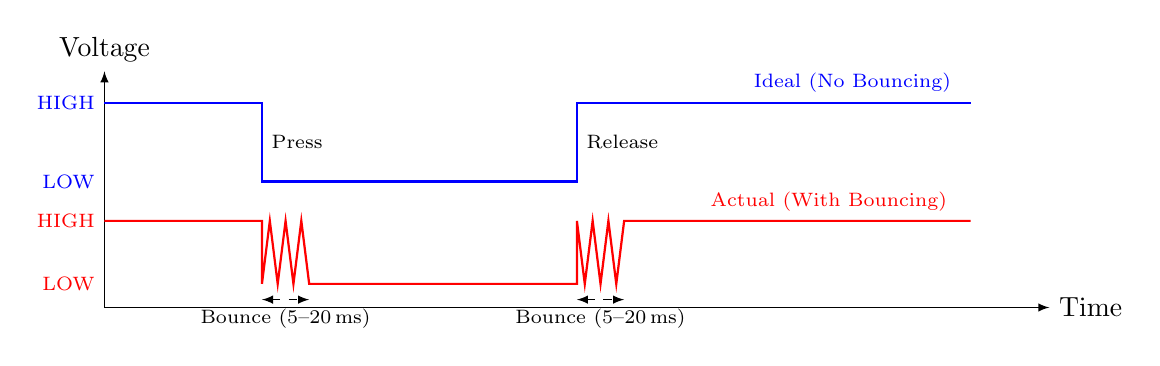
\begin{tikzpicture}[x=1cm,y=1cm,>=latex]
  % Axes
  \draw[->] (0,0) -- (12,0) node[right]{Time};
  \draw[->] (0,0) -- (0,3) node[above]{Voltage};

  % --- Ideal signal lane (upper) ---
  % Levels for the upper lane
  \def\HIGHU{2.6}
  \def\LOWU{1.6}
  % Ideal (no bounce)
  \draw[thick, blue]
    (0,\HIGHU) -- (2,\HIGHU)
    -- (2,\LOWU)
    -- (6,\LOWU)
    -- (6,\HIGHU)
    -- (11,\HIGHU);
  \node[blue] at (9.5,2.85) {\scriptsize Ideal (No Bouncing)};
  \node[blue, anchor=east] at (0,\HIGHU) {\scriptsize HIGH};
  \node[blue, anchor=east] at (0,\LOWU) {\scriptsize LOW};

  % --- Actual signal lane (lower) ---
  % Levels for the lower lane
  \def\HIGHL{1.1}
  \def\LOWL{0.3}
  % Actual with bounce (press and release)
  \draw[thick, red]
    (0,\HIGHL) -- (2,\HIGHL)
    % Press bounce
    -- (2,\LOWL)
    -- (2.10,\HIGHL)
    -- (2.20,\LOWL)
    -- (2.30,\HIGHL)
    -- (2.40,\LOWL)
    -- (2.50,\HIGHL)
    -- (2.60,\LOWL)
    -- (6,\LOWL)
    % Release bounce
    -- (6,\HIGHL)
    -- (6.10,\LOWL)
    -- (6.20,\HIGHL)
    -- (6.30,\LOWL)
    -- (6.40,\HIGHL)
    -- (6.50,\LOWL)
    -- (6.60,\HIGHL)
    -- (11,\HIGHL);
  \node[red] at (9.2,1.35) {\scriptsize Actual (With Bouncing)};
  \node[red, anchor=east] at (0,\HIGHL) {\scriptsize HIGH};
  \node[red, anchor=east] at (0,\LOWL) {\scriptsize LOW};

  % Bounce duration brackets
  \draw[<->, dashed] (2,0.1) -- (2.6,0.1)
    node[midway, below]{\scriptsize Bounce (5--20\,ms)};
  \draw[<->, dashed] (6,0.1) -- (6.6,0.1)
    node[midway, below]{\scriptsize Bounce (5--20\,ms)};

  % Transition labels
  \node[anchor=west] at (2,2.1) {\scriptsize Press};
  \node[anchor=west] at (6,2.1) {\scriptsize Release};
\end{tikzpicture}
\caption{Mechanical Switch Bounce — Press and Release Both Exhibit Bouncing}
\end{figure}


\noindent
For applications that poll the input at a slow rate or only care about the final state, bouncing may not be a problem. However, for interrupt-driven systems or applications that count button presses, bouncing can cause multiple false triggers.

\subsubsection{Debouncing Techniques}

Two approaches can eliminate or mitigate switch bouncing:

\paragraph{Hardware Debouncing}
Add an RC (resistor-capacitor) filter circuit or a dedicated debouncing IC to the switch. The capacitor smooths out the voltage transitions, preventing bounces from reaching the microcontroller input.

\paragraph{Software Debouncing}
After detecting a button press (or release), wait for a short period (typically 10-50 ms) to allow the bouncing to settle, then read the input again to confirm the state. This can be implemented with:
\begin{itemize}[nosep]
  \item \textbf{Blocking delay debouncing}: Insert a fixed delay (busy-wait loop) after detecting an edge, then verify the input state. This is simple but prevents the CPU from doing other work during the delay period.
  \item \textbf{Timer-based debouncing (non-blocking)}: Use a hardware timer to sample the input periodically without blocking the main program. Only register a press after multiple consistent readings across timer intervals.
\end{itemize}

\noindent
For this experiment, we will implement simple delay-based debouncing in our polling examples. More sophisticated timer-based debouncing techniques will be covered in the following experiment.

\subsection{Reading GPIO Inputs: Polling vs. Interrupts}

There are two fundamental approaches to reading digital inputs:

\subsubsection{Polling (Continuous Checking)}

In polling, the CPU continuously reads the input pin in a loop and checks whether the state has changed. This is simple to implement but has drawbacks:

\begin{itemize}[nosep]
  \item \textbf{CPU Usage}: The CPU is busy checking the input even when nothing is happening.
  \item \textbf{Latency}: The response time depends on how frequently the loop runs.
  \item \textbf{Power Consumption}: The CPU cannot enter low-power sleep modes while polling.
\end{itemize}

\noindent
Polling is suitable for simple applications where the CPU has nothing else to do or when inputs change slowly.

\begin{lstlisting}[caption={Polling Example (Conceptual)}, language=C]
while (1) {
    if (button is pressed) {
        // Respond to button press
    }
}
\end{lstlisting}

\subsubsection{Interrupts (Event-Driven Response)}

In interrupt-driven input, the GPIO peripheral notifies the CPU when an input change occurs by generating an \textbf{interrupt request} (IRQ). The CPU immediately stops its current task, executes an \textbf{Interrupt Service Routine} (ISR), and then resumes normal operation.

\begin{itemize}[nosep]
  \item \textbf{Efficiency}: The CPU can do other work or sleep until an input event occurs.
  \item \textbf{Responsiveness}: The CPU reacts immediately to input changes.
  \item \textbf{Power Efficiency}: The CPU can remain in low-power modes and wake only when needed.
\end{itemize}

\noindent
Interrupts are essential for responsive embedded systems and are the preferred method for handling asynchronous events.

\begin{lstlisting}[caption={Interrupt Example (Conceptual)}, language=C]
// Main loop can perform other tasks
while (1) {
    // Do other work or sleep
}

// ISR is called automatically when button is pressed
void ButtonISR(void) {
    // Respond to button press
    // Clear interrupt flag
}
\end{lstlisting}

\subsection{How Interrupts Work}

Understanding the interrupt mechanism is essential for writing interrupt-driven programs. This section explains the complete lifecycle of an interrupt from trigger to completion.

\subsubsection{Interrupt Lifecycle}

When a GPIO pin configured for interrupts detects the specified event (e.g., a button press), the following sequence occurs:

\paragraph{1. Event Detection}
The GPIO peripheral continuously monitors the pin according to its configuration (edge/level detection). When the configured condition is met (e.g., falling edge), the peripheral sets an internal flag.

\paragraph{2. Interrupt Request (IRQ)}
If the interrupt is unmasked (enabled in \texttt{GPIOIM}), the GPIO module sends an interrupt request to the NVIC. The NVIC receives interrupt requests from all peripherals and manages their execution.

\paragraph{3. CPU Response}
The NVIC checks if the interrupt is enabled (\texttt{NVIC\_ISER}) and compares its priority with currently executing code. If the interrupt should be serviced:
\begin{itemize}[nosep]
  \item The CPU finishes executing the current instruction.
  \item The CPU automatically saves the current execution context (program counter, registers, status flags) onto the stack.
  \item The CPU loads the address of the Interrupt Service Routine (ISR) from the vector table.
  \item Execution jumps to the ISR.
\end{itemize}

\paragraph{4. ISR Execution}
The ISR (e.g., \texttt{GPIOF\_Handler()}) executes and must:
\begin{itemize}[nosep]
  \item Identify which pin(s) caused the interrupt (read \texttt{GPIOMIS}).
  \item Perform the required response (toggle LED, set flag, etc.).
  \item Clear the interrupt flag (write to \texttt{GPIOICR}) — \textbf{critical step}.
\end{itemize}

\paragraph{5. Return from Interrupt}
When the ISR completes (returns), the CPU:
\begin{itemize}[nosep]
  \item Automatically restores the saved context from the stack.
  \item Resumes execution from where it was interrupted.
\end{itemize}

\noindent
This entire process happens in microseconds, making interrupts extremely responsive.

\subsubsection{Why Clear the Interrupt Flag?}

The interrupt flag remains set until explicitly cleared by software. If the ISR does not clear the flag by writing to \texttt{GPIOICR}, the NVIC will immediately re-trigger the interrupt as soon as the ISR returns, creating an infinite loop of interrupts that hangs the system.

\begin{lstlisting}[caption={Critical: Always clear the interrupt flag}, language=C]
void GPIOF_Handler(void) {
    // Read which pin caused interrupt
    if (GPIOF->MIS & (1 << 4)) {
        // Handle PF4 interrupt
        // ...
        
        GPIOF->ICR |= (1 << 4);  // MUST clear flag!
    }
}
\end{lstlisting}

\subsubsection{Interrupt Advantages and Considerations}

\paragraph{Advantages:}
\begin{itemize}[nosep]
  \item \textbf{Efficient}: CPU can perform other tasks or sleep while waiting for events.
  \item \textbf{Responsive}: Immediate response to external events (microsecond latency).
  \item \textbf{Power-efficient}: CPU can remain in low-power modes between events.
  \item \textbf{Real-time}: Predictable timing for critical events.
\end{itemize}

\paragraph{Considerations:}
\begin{itemize}[nosep]
  \item \textbf{Complexity}: More complex to implement and debug than polling.
  \item \textbf{Shared data}: ISRs and main code must carefully manage shared variables (use \texttt{volatile}).
  \item \textbf{ISR constraints}: ISRs should be short and fast — avoid delays and lengthy operations.
  \item \textbf{Debouncing}: Mechanical switch bouncing can trigger multiple interrupts; software or hardware debouncing is often necessary.
\end{itemize}

\subsection{GPIO Input Configuration Registers}


Before a GPIO pin can be used as an input, it must first be configured for digital functionality.  
As discussed in the previous experiment, the following three steps are required for \textbf{all GPIO pins}:
\medskip
\begin{enumerate}[nosep]
  \item \textbf{Enable the GPIO clock} via \texttt{SYSCTL\_RCGCGPIO}.
  \item \textbf{Select the direction} of the pin using \texttt{GPIO\_DIR}  
        (\texttt{0} for input, \texttt{1} for output).
  \item \textbf{Enable digital functionality} using \texttt{GPIO\_DEN}.
\end{enumerate}
\medskip
Once a pin is set as an input, the logic level on the pin may be undefined if it is left floating (not driven by an external source).  
To ensure a stable logic level, internal resistors can be activated:
\medskip
These resistors are controlled by two dedicated registers:
\begin{itemize}[nosep]
  \item \texttt{GPIO\_PUR} — Enable internal pull-up resistor on the selected pin(s).
  \item \texttt{GPIO\_PDR} — Enable internal pull-down resistor on the selected pin(s).
\end{itemize}

\subsubsection*{GPIOPUR — Pull-Up Resistor Enable}

\noindent\textbf{Register:} \texttt{GPIOPUR} — GPIO Pull-Up Select (Port F: \texttt{0x40025510})

\noindent
The \texttt{GPIOPUR} register enables the internal pull-up resistor for each GPIO pin. When enabled, the pin is weakly pulled to logic '1' (3.3V) through a resistor (typically 13-40 k$\omega$). This prevents floating inputs and is essential for switches connected to ground.

\begin{figure}[H]
\centering
\begin{bytefield}[endianness=big,bitwidth=\widthof{~PF7~}]{16}
\bitheader[lsb=16]{16-31} \\
\bitbox{16}[bgcolor=gray!10]{\tiny{reserved}} \\
\bitheader{0-15} \\
\bitbox{8}[bgcolor=gray!10]{\tiny{reserved}} & \bitbox{1}{PF7} & \bitbox{1}{PF6} & \bitbox{1}{PF5} & \bitbox{1}{PF4} & \bitbox{1}{PF3} & \bitbox{1}{PF2} & \bitbox{1}{PF1} & \bitbox{1}{PF0}
\end{bytefield}
\caption{GPIOPUR Register — Pull-Up Enable}
\end{figure}

\noindent
\textbf{Bit Values:}
\begin{itemize}[nosep]
  \item \textbf{0}: Pull-up disabled (default)
  \item \textbf{1}: Pull-up enabled
\end{itemize}

\noindent
For the LaunchPad switches (SW1 on PF4, SW2 on PF0), pull-ups must be enabled.

\bigskip
\subsubsection*{GPIOPDR — Pull-Down Resistor Enable}

\noindent\textbf{Register:} \texttt{GPIOPDR} — GPIO Pull-Down Select (Port F: \texttt{0x40025514})

\noindent
The \texttt{GPIOPDR} register enables the internal pull-down resistor for each GPIO pin. When enabled, the pin is weakly pulled to logic '0' (0V) through a resistor. This is used for switches connected to power (\texttt{VCC}).

\begin{figure}[H]
\centering
\begin{bytefield}[endianness=big,bitwidth=\widthof{~PF7~}]{16}
\bitheader[lsb=16]{16-31} \\
\bitbox{16}[bgcolor=gray!10]{\tiny{reserved}} \\
\bitheader{0-15} \\
\bitbox{8}[bgcolor=gray!10]{\tiny{reserved}} & \bitbox{1}{PF7} & \bitbox{1}{PF6} & \bitbox{1}{PF5} & \bitbox{1}{PF4} & \bitbox{1}{PF3} & \bitbox{1}{PF2} & \bitbox{1}{PF1} & \bitbox{1}{PF0}
\end{bytefield}
\caption{GPIOPDR Register — Pull-Down Enable}
\end{figure}

\noindent
\textbf{Bit Values:}
\begin{itemize}[nosep]
  \item \textbf{0}: Pull-down disabled (default)
  \item \textbf{1}: Pull-down enabled
\end{itemize}

\noindent
\textbf{Note:} Pull-up and pull-down resistors should not be enabled simultaneously on the same pin.
\subsection{Unlocking Protected GPIO Pins}

Some GPIO pins on the TM4C123 are \textbf{locked} by default to prevent accidental reconfiguration of critical functions such as JTAG/SWD (debug interface) and NMI (Non-Maskable Interrupt).

On Port F, pin \textbf{PF0} is locked because it is the NMI input by default. To use PF0 as a general-purpose GPIO input (for SW2 on the LaunchPad), it must be unlocked.

\subsubsection*{GPIOLOCK — Lock Register}

\noindent\textbf{Register:} \texttt{GPIOLOCK} — GPIO Lock (Port F: \texttt{0x40025520})

\noindent
The \texttt{GPIOLOCK} register controls write access to the \texttt{GPIOCR} register. Writing the magic value \texttt{0x4C4F434B} ("LOCK" in ASCII) unlocks the port and allows modifications to the commit register.


\noindent
\textbf{Values:}
\begin{itemize}[nosep]
  \item Write \texttt{0x4C4F434B}: Unlock the port (allow changes to \texttt{GPIOCR})
  \item Write any other value: Lock the port (prevent changes to \texttt{GPIOCR})
  \item Read: Returns \texttt{0x00000001} if locked, \texttt{0x00000000} if unlocked
\end{itemize}

\bigskip
\subsubsection*{GPIOCR — Commit Register}

\noindent\textbf{Register:} \texttt{GPIOCR} — GPIO Commit (Port F: \texttt{0x40025524})

\noindent
The \texttt{GPIOCR} register controls which pins can be reconfigured. After unlocking with \texttt{GPIOLOCK}, set the corresponding bit in \texttt{GPIOCR} to allow changes to that pin's configuration registers.

\begin{figure}[H]
\centering
\begin{bytefield}[endianness=big,bitwidth=\widthof{~PF7~}]{16}
\bitheader[lsb=16]{16-31} \\
\bitbox{16}[bgcolor=gray!10]{\tiny{reserved}} \\
\bitheader{0-15} \\
\bitbox{8}[bgcolor=gray!10]{\tiny{reserved}} & \bitbox{1}{PF7} & \bitbox{1}{PF6} & \bitbox{1}{PF5} & \bitbox{1}{PF4} & \bitbox{1}{PF3} & \bitbox{1}{PF2} & \bitbox{1}{PF1} & \bitbox{1}{PF0}
\end{bytefield}
\caption{GPIOCR Register — Commit Control}
\end{figure}

\noindent
\textbf{Bit Values:}
\begin{itemize}[nosep]
  \item \textbf{0}: Pin configuration is locked (cannot be modified)
  \item \textbf{1}: Pin configuration is unlocked (can be modified)
\end{itemize}

\bigskip
\subsubsection*{Unlocking Procedure}

To unlock a protected pin (such as PF0):

\begin{enumerate}[nosep]
  \item Write the unlock key \texttt{0x4C4F434B} to the \texttt{GPIOLOCK} register.
  \item Set the corresponding bit in the \texttt{GPIOCR} (Commit Register) to allow changes.
  \item Configure the pin normally (\texttt{GPIODIR}, \texttt{GPIODEN}, etc.).
\end{enumerate}

\begin{lstlisting}[caption={Unlocking PF0 for GPIO use}, language=C]
GPIOF->LOCK = 0x4C4F434B;    // Unlock Port F
GPIOF->CR   |= (1 << 0);     // Allow changes to PF0
\end{lstlisting}

\noindent
After unlocking, PF0 can be configured like any other GPIO pin.

\bigskip
\subsection{GPIO Interrupt Configuration Registers}

To configure a GPIO pin to generate interrupts, several registers must be configured. The process involves selecting the trigger condition (edge or level, rising or falling) and enabling the interrupt at both the GPIO module and the NVIC.

\subsubsection*{GPIOIS — Interrupt Sense Register}

\noindent\textbf{Register:} \texttt{GPIOIS} — GPIO Interrupt Sense (Port F: \texttt{0x40025404})

\noindent
The \texttt{GPIOIS} register determines whether interrupts are triggered by signal \textbf{edges} (transitions) or \textbf{levels} (steady states).

\begin{figure}[H]
\centering
\begin{bytefield}[endianness=big,bitwidth=\widthof{~PF7~}]{16}
\bitheader[lsb=16]{16-31} \\
\bitbox{16}[bgcolor=gray!10]{\tiny{reserved}} \\
\bitheader{0-15} \\
\bitbox{8}[bgcolor=gray!10]{\tiny{reserved}} & \bitbox{1}{PF7} & \bitbox{1}{PF6} & \bitbox{1}{PF5} & \bitbox{1}{PF4} & \bitbox{1}{PF3} & \bitbox{1}{PF2} & \bitbox{1}{PF1} & \bitbox{1}{PF0}
\end{bytefield}
\caption{GPIOIS Register — Interrupt Sense}
\end{figure}

\noindent
\textbf{Bit Values:}
\begin{itemize}[nosep]
  \item \textbf{0}: Edge-sensitive (detects transitions) — typical for buttons
  \item \textbf{1}: Level-sensitive (detects steady state)
\end{itemize}

\bigskip
\subsubsection*{GPIOIBE — Interrupt Both Edges Register}

\noindent\textbf{Register:} \texttt{GPIOIBE} — GPIO Interrupt Both Edges (Port F: \texttt{0x40025408})

\noindent
When edge-sensitive mode is selected (bit cleared in \texttt{GPIOIS}), this register determines whether interrupts occur on a single edge or both edges.

\begin{figure}[H]
\centering
\begin{bytefield}[endianness=big,bitwidth=\widthof{~PF7~}]{16}
\bitheader[lsb=16]{16-31} \\
\bitbox{16}[bgcolor=gray!10]{\tiny{reserved}} \\
\bitheader{0-15} \\
\bitbox{8}[bgcolor=gray!10]{\tiny{reserved}} & \bitbox{1}{PF7} & \bitbox{1}{PF6} & \bitbox{1}{PF5} & \bitbox{1}{PF4} & \bitbox{1}{PF3} & \bitbox{1}{PF2} & \bitbox{1}{PF1} & \bitbox{1}{PF0}
\end{bytefield}
\caption{GPIOIBE Register — Interrupt Both Edges}
\end{figure}

\noindent
\textbf{Bit Values:}
\begin{itemize}[nosep]
  \item \textbf{0}: Single edge (rising or falling, defined by \texttt{GPIOIEV})
  \item \textbf{1}: Both rising and falling edges trigger interrupts
\end{itemize}

\bigskip
\subsubsection*{GPIOIEV — Interrupt Event Register}

\noindent\textbf{Register:} \texttt{GPIOIEV} — GPIO Interrupt Event (Port F: \texttt{0x4002540C})

\noindent
For single-edge interrupts (when the corresponding bit in \texttt{GPIOIBE} is 0), this register selects which edge triggers the interrupt.

\begin{figure}[H]
\centering
\begin{bytefield}[endianness=big,bitwidth=\widthof{~PF7~}]{16}
\bitheader[lsb=16]{16-31} \\
\bitbox{16}[bgcolor=gray!10]{\tiny{reserved}} \\
\bitheader{0-15} \\
\bitbox{8}[bgcolor=gray!10]{\tiny{reserved}} & \bitbox{1}{PF7} & \bitbox{1}{PF6} & \bitbox{1}{PF5} & \bitbox{1}{PF4} & \bitbox{1}{PF3} & \bitbox{1}{PF2} & \bitbox{1}{PF1} & \bitbox{1}{PF0}
\end{bytefield}
\caption{GPIOIEV Register — Interrupt Event}
\end{figure}

\noindent
\textbf{Bit Values:}
\begin{itemize}[nosep]
  \item \textbf{0}: Falling edge (high-to-low transition)
  \item \textbf{1}: Rising edge (low-to-high transition)
\end{itemize}

\noindent
For switches with pull-ups (LaunchPad SW1/SW2), falling edge interrupts detect button presses.

\bigskip
\subsubsection*{GPIOIM — Interrupt Mask Register}

\noindent\textbf{Register:} \texttt{GPIOIM} — GPIO Interrupt Mask (Port F: \texttt{0x40025410})

\noindent
The \texttt{GPIOIM} register enables or disables (masks/unmasks) interrupt generation for each pin. Setting a bit to '1' allows that pin to generate interrupts.

\begin{figure}[H]
\centering
\begin{bytefield}[endianness=big,bitwidth=\widthof{~PF7~}]{16}
\bitheader[lsb=16]{16-31} \\
\bitbox{16}[bgcolor=gray!10]{\tiny{reserved}} \\
\bitheader{0-15} \\
\bitbox{8}[bgcolor=gray!10]{\tiny{reserved}} & \bitbox{1}{PF7} & \bitbox{1}{PF6} & \bitbox{1}{PF5} & \bitbox{1}{PF4} & \bitbox{1}{PF3} & \bitbox{1}{PF2} & \bitbox{1}{PF1} & \bitbox{1}{PF0}
\end{bytefield}

\caption{GPIOIM Register — Interrupt Mask}
\end{figure}

\noindent
\textbf{Bit Values:}
\begin{itemize}[nosep]
  \item \textbf{0}: Interrupt disabled (masked) — default
  \item \textbf{1}: Interrupt enabled (unmasked)
\end{itemize}

\bigskip
\subsubsection*{GPIOMIS — Masked Interrupt Status Register}

\noindent\textbf{Register:} \texttt{GPIOMIS} — GPIO Masked Interrupt Status (Port F: \texttt{0x40025418})

\noindent
This read-only register shows which pins have pending interrupts after masking. The ISR reads this register to determine which pin(s) caused the interrupt.

\begin{figure}[H]
\centering
\begin{bytefield}[endianness=big,bitwidth=\widthof{~PF7~}]{16}
\bitheader[lsb=16]{16-31} \\
\bitbox{16}[bgcolor=gray!10]{\tiny{reserved}} \\
\bitheader{0-15} \\
\bitbox{8}[bgcolor=gray!10]{\tiny{reserved}} & \bitbox{1}{PF7} & \bitbox{1}{PF6} & \bitbox{1}{PF5} & \bitbox{1}{PF4} & \bitbox{1}{PF3} & \bitbox{1}{PF2} & \bitbox{1}{PF1} & \bitbox{1}{PF0}
\end{bytefield}
\caption{GPIOMIS Register — Masked Interrupt Status (Read-Only)}
\end{figure}

\noindent
\textbf{Bit Values:}
\begin{itemize}[nosep]
  \item \textbf{0}: No interrupt pending for this pin
  \item \textbf{1}: Interrupt pending for this pin
\end{itemize}

\bigskip
\subsubsection*{GPIOICR — Interrupt Clear Register}

\noindent\textbf{Register:} \texttt{GPIOICR} — GPIO Interrupt Clear (Port F: \texttt{0x4002541C})

\noindent
Writing '1' to a bit in this register clears the corresponding interrupt flag. This is \textbf{critical}: the ISR must clear the flag, or the interrupt will continuously re-trigger.

\begin{figure}[H]
\centering
\begin{bytefield}[endianness=big,bitwidth=\widthof{~PF7~}]{16}
\bitheader[lsb=16]{16-31} \\
\bitbox{16}[bgcolor=gray!10]{\tiny{reserved}} \\
\bitheader{0-15} \\
\bitbox{8}[bgcolor=gray!10]{\tiny{reserved}} & \bitbox{1}{PF7} & \bitbox{1}{PF6} & \bitbox{1}{PF5} & \bitbox{1}{PF4} & \bitbox{1}{PF3} & \bitbox{1}{PF2} & \bitbox{1}{PF1} & \bitbox{1}{PF0}
\end{bytefield}
\caption{GPIOICR Register — Interrupt Clear}
\end{figure}

\noindent
\textbf{Bit Values:}
\begin{itemize}[nosep]
  \item Write \textbf{1} to clear the interrupt flag for that pin
  \item Write \textbf{0} has no effect
\end{itemize}

\bigskip
\subsection{Configuration Workflow}

GPIO interrupt configuration is divided into two parts, configuring the pin as an input and configuring the interrupt settings. The following steps summarize the process:

\paragraph{Step 1: Pin Configuration}
Configure the GPIO pin as an input with proper electrical characteristics:
\begin{enumerate}[nosep]
  \item Enable the GPIO port clock (\texttt{RCGCGPIO}).
  \item Unlock protected pins if needed (\texttt{GPIOLOCK}, \texttt{GPIOCR}).
  \item Configure the pin as input (\texttt{GPIODIR} = 0).
  \item Enable the digital function (\texttt{GPIODEN} = 1).
  \item Enable pull-up or pull-down resistor (\texttt{GPIOPUR} or \texttt{GPIOPDR}).
\end{enumerate}

\paragraph{Step 2: Interrupt Configuration}
\begin{enumerate}[nosep]
  \item Configure interrupt sense (\texttt{GPIOIS} = 0 for edge-sensitive).
  \item Select edge(s) (\texttt{GPIOIBE}/\texttt{GPIOIEV}).
  \item \textbf{Clear any prior flags} (\texttt{GPIOICR} = 1 for the pin).
  \item Unmask the pin in the GPIO (\texttt{GPIOIM} = 1).
  \item Enable the IRQ in the NVIC.
\end{enumerate}


\subsection{NVIC — Nested Vectored Interrupt Controller}

The NVIC manages all peripheral interrupts on the Cortex-M4, deciding which ISR to execute based on enable bits, masking, and priority.

\subsubsection*{NVIC\_ISER — Interrupt Set-Enable Registers}

\noindent\textbf{Registers:} \texttt{NVIC\_ISER[0..3]} (\texttt{0xE000E100-0xE000E10C})

\noindent
Each 32-bit \texttt{ISER} register enables up to 32 interrupt sources.  
Writing a '1' to a bit enables that IRQ; writing '0' has no effect.

\begin{table}[H]
\centering
\small
\renewcommand{\arraystretch}{1.1}
\begin{tabular}{lll}
\toprule
\textbf{Register} & \textbf{IRQ Range} & \textbf{Address} \\
\midrule
\texttt{ISER[0]} & 0-31  & 0xE000E100 \\
\texttt{ISER[1]} & 32-63 & 0xE000E104 \\
\texttt{ISER[2]} & 64-95 & 0xE000E108 \\
\texttt{ISER[3]} & 96-127 & 0xE000E10C \\
\bottomrule
\end{tabular}
\caption{Interrupt ranges for NVIC\_ISER registers}
\end{table}

\noindent
For the TM4C123, all GPIO interrupts (IRQ0-IRQ4) for Ports A-E, and Port F (IRQ30) are in \texttt{ISER[0]}.
\bigskip


\noindent
\textbf{Example — Enabling Port F Manually}
\begin{lstlisting}[caption={Enable GPIO Port F interrupt manually}, language=C]
NVIC->ISER[0] |= (1 << 30);   // IRQ30 - NVIC_EN0 bit 30
\end{lstlisting}

\noindent
\textbf{CMSIS Alternative (Recommended):}
\begin{lstlisting}[language=C]
NVIC_EnableIRQ(GPIOF_IRQn);
\end{lstlisting}

\noindent
This function automatically computes the correct register and bit:
\begin{lstlisting}[language=C]
void NVIC_EnableIRQ(IRQn_Type IRQn) {
    if (IRQn >= 0)
        NVIC->ISER[IRQn >> 5] |= (1u << (IRQn & 0x1F)); // /32 and %32
}
\end{lstlisting}
\noindent
\paragraph{Explanation:}
\[
\text{Register index} = \left\lfloor \frac{\text{IRQn}}{32} \right\rfloor, \qquad
\text{Bit position} = \text{IRQn} \bmod 32.
\]

\noindent
Each \texttt{ISER} register enables 32 interrupts.  
Dividing the IRQ number by 32 selects the correct register index, and the remainder (\texttt{IRQn \% 32}) identifies the bit position within that 32-bit register.
\subsection{Interrupt Service Routine (ISR)}

When a GPIO interrupt occurs, the NVIC calls the corresponding ISR. For GPIO Port F, the ISR is named \texttt{GPIOF\_Handler()}. The ISR must:

\begin{enumerate}[nosep]
  \item Determine which pin caused the interrupt (read \texttt{GPIOMIS}).
  \item Perform the required action (e.g., toggle an LED).
  \item Clear the interrupt flag (write to \texttt{GPIOICR}).
\end{enumerate}

\begin{lstlisting}[caption={GPIO Port F ISR Template}, language=C]
void GPIOF_Handler(void) {
    if (GPIOF->MIS & (1 << 4)) {     // Check if PF4 caused interrupt
        // Respond to SW1 press
        GPIOF->ICR |= (1 << 4);      // Clear PF4 interrupt flag
    }
    if (GPIOF->MIS & (1 << 0)) {     // Check if PF0 caused interrupt
        // Respond to SW2 press
        GPIOF->ICR |= (1 << 0);      // Clear PF0 interrupt flag
    }
}
\end{lstlisting}


\newpage
\section{Procedure}

\subsection{Examples}

The following examples demonstrate GPIO input configuration using polling and interrupt-based approaches.

\subsubsection{Example 1 — Reading Switch Input Using Polling}

This example continuously polls the state of SW1 (PF4) and turns on the red LED (PF1) when the button is pressed.

\lstinputlisting[language=C, caption={Polling-based switch input reading}]{snippets/gpio/polling.c}

\noindent
\textbf{Explanation:}
\begin{itemize}[nosep]
  \item \texttt{GPIOF->PUR |= SWITCH;} enables the internal pull-up resistor on PF4.
  \item The \texttt{while(1)} loop continuously reads the switch state.
  \item When \texttt{state == 0}, the button is pressed (pull-up makes it active-low).
  \item The LED is controlled directly in the main loop without interrupts.
\end{itemize}
\newpage
\subsubsection{Example 2 — Interrupt-Driven Switch Input}

This example configures SW1 and SW2 to generate interrupts on button presses and toggles the green LED in the ISR.

\lstinputlisting[language=C, caption={Interrupt-driven switch input handling}]{snippets/gpio/interrupt.c}

\noindent
\textbf{Explanation:}
\begin{itemize}[nosep]
  \item \texttt{GPIOF->LOCK = 0x4C4F434B;} unlocks Port F for PF0 configuration.
  \item \texttt{GPIOF->CR = 0x01;} allows changes to PF0.
  \item \texttt{GPIOF->IS \&= \textasciitilde(SW1 | SW2);} configures edge-sensitive interrupts.
  \item \texttt{GPIOF->IEV \&= \textasciitilde(SW1 | SW2);} selects falling-edge trigger (button press).
  \item \texttt{GPIOF->ICR |= (SW1 | SW2);} clears any prior interrupt flags before enabling.
  \item \texttt{GPIOF->IM |= (SW1 | SW2);} unmasks (enables) interrupts for SW1 and SW2.
  \item \texttt{NVIC->ISER[0] |= (1<<30);} enables GPIO Port F interrupt in NVIC.
  \item The ISR checks \texttt{GPIOF->MIS} to identify which switch caused the interrupt.
  \item Each interrupt flag must be cleared with \texttt{GPIOF->ICR} to prevent re-triggering.
\end{itemize}
\newpage
\subsection{Tasks}

\subsubsection{Task 1 — Toggle LED Using Polling}

Modify Example 1 to toggle the green LED (PF3) with each press of SW1 (PF4). The LED should change state (ON→OFF or OFF→ON) every time the button is pressed and released.

\paragraph{Requirements:}
\begin{itemize}[nosep]
  \item Use polling to detect button presses.
  \item Implement software debouncing by adding a delay after detecting a press.
  \item Toggle the LED state instead of simply turning it on or off.
  \item Ensure the LED changes state only once per button press.
\end{itemize}

\medskip


\subsubsection{Task 2 — LED Sequence Using Interrupts}

Modify Example 2 to cycle through LED colors using interrupts:
\begin{itemize}[nosep]
  \item Pressing SW1 (PF4) cycles through: \textbf{Red → Blue → Green → Red...}
  \item Pressing SW2 (PF0) cycles through: \textbf{Yellow → Magenta → Cyan → Yellow...}
\end{itemize}

\paragraph{Requirements:}
\begin{itemize}[nosep]
  \item Use interrupt-driven input handling.
  \item Maintain separate state variables for each button's LED sequence.
  \item Update the LED color in the ISR based on the current state.
  \item Clear interrupt flags properly to avoid repeated triggering.
\end{itemize}

\paragraph{Hint:}
Use a global variable (e.g., \texttt{sw1\_state}) to track the current position in the sequence. In the ISR, increment the state and use a switch-case or modulo operation to cycle through colors. Refer to Table~\ref{tab:led-colors} in Experiment 4 for LED color codes.
\chapter{Hardware Timers and Timing Control}

\section*{Learning Objectives}
After completing this experiment, you will be able to:
\begin{itemize}[nosep]
  \item Understand the role and limitations of the SysTick timer in the ARM Cortex-M4 core.
  \item Configure the SysTick timer for periodic interrupts and precise timing.
  \item Understand the architecture and capabilities of General-Purpose Timer Modules (GPTM).
  \item Configure GPTM in 16-bit and 32-bit modes for periodic and one-shot operation.
  \item Calculate timer periods using prescalers and reload values.
  \item Implement timer-based debouncing for mechanical switches.
  \item Use multiple timers to control independent timing tasks.
\end{itemize}

\section*{Experiment Overview}
This experiment introduces precise timing control using the TM4C123's SysTick timer and General-Purpose Timer Modules (GPTM). You will configure SysTick for periodic interrupts and millisecond timing, explore GPTM's 16-bit and 32-bit modes with prescalers, and implement multiple independent timing tasks. By the end of this lab, you will understand how to select and configure timers for different timing requirements and implement timer-based interrupt-driven applications.

\newpage
\etocsetnexttocdepth{subsubsection}
\localtableofcontents
\bigskip
\newpage



\section{Theoretical Background}
\subsection{Clock Sources}

Unless otherwise noted, we assume the \textbf{System Clock (SysClk) = 50\,MHz} for all calculations in this chapter.

\subsubsection{Clock Setup in Keil µVision5}

When you create a project in Keil µVision5 for the TM4C123, the \textbf{startup file} (\texttt{startup\_TM4C123.s}) and \textbf{system initialization code} (\texttt{system\_TM4C123.c}) automatically configure the system clock to 50\,MHz. This setup occurs before \texttt{main()} is called and:

\begin{itemize}[nosep]
  \item Enables the PLL (Phase-Locked Loop) to multiply the crystal oscillator frequency
  \item Configures the system divider to achieve the target 50\,MHz frequency
  \item Sets the \texttt{SystemCoreClock} variable to \texttt{50000000} for use in CMSIS functions like \texttt{SysTick\_Config()}
\end{itemize}

\noindent
You can verify the clock configuration by checking the value of \texttt{SystemCoreClock} in your code or by examining the \texttt{SystemInit()} function in \texttt{system\_TM4C123.c}.

\subsubsection{System Clock on TM4C123}

The system clock can be derived from multiple sources:

\begin{itemize}[nosep]
  \item \textbf{MOSC}: Main oscillator (external crystal, typically 16\,MHz or 25\,MHz)
  \item \textbf{PIOSC}: Precision internal oscillator (16\,MHz $\pm$ 1\%)
  \item \textbf{PIOSC/4}: Internal oscillator divided by 4 ($\approx$ 4\,MHz)
  \item \textbf{LFIOSC}: Low-frequency internal oscillator ($\sim$30\,kHz)
  \item \textbf{PLL}: Phase-Locked Loop (can multiply oscillator frequency)
\end{itemize}

\noindent
Peripherals, including GPTM, are clocked from the system clock (SysClk) once enabled in the \texttt{RCGCTIMER} register. The Keil startup file typically configures the PLL to generate 50\,MHz from a 16\,MHz crystal.

\subsubsection{SysTick Clock Source}

The SysTick timer can use one of two clock sources, selected via the \texttt{CLKSOURCE} bit in the \texttt{CTRL} register:

\begin{itemize}[nosep]
  \item \textbf{Processor clock} (bit = 1): Same as system clock (50\,MHz in our case)
  \item \textbf{Reference clock} (bit = 0): Typically PIOSC/4 ($\approx$ 4\,MHz), useful for a stable timebase independent of PLL changes
\end{itemize}

\noindent
For this lab, we use the processor clock (50\,MHz) for both SysTick and GPTM.

\subsection{How Timers Work}

Understanding the basic operation of timers will help you configure them correctly and debug timing issues.

\subsubsection{Down-Counting Operation}

Both SysTick and GPTM timers operate as \textbf{down-counters} in their most common configuration (periodic mode):

\begin{enumerate}[nosep]
  \item \textbf{Load}: A reload value is written to the timer's load register (\texttt{LOAD} for SysTick, \texttt{TAILR} for GPTM)
  \item \textbf{Count}: The timer counts down from the reload value to zero, decrementing once per clock cycle (or prescaled cycle)
  \item \textbf{Timeout}: When the counter reaches zero:
    \begin{itemize}[nosep]
      \item The timeout flag is set
      \item An interrupt is generated (if enabled and unmasked)
      \item The counter automatically reloads from the load register (periodic mode) or stops (one-shot mode)
    \end{itemize}
  \item \textbf{Clear}: The interrupt handler must clear the timeout flag by writing to the interrupt clear register
\end{enumerate}

\subsubsection{Timer Modes}

Timers can operate in different modes depending on the application:

\begin{itemize}[nosep]
  \item \textbf{Periodic Mode}: The timer automatically reloads and continues counting. Ideal for fixed-rate tasks like LED blinking, sampling sensors, or OS ticks.
  \item \textbf{One-Shot Mode}: The timer counts down once and stops. Useful for timeouts, delays, or single events.
  \item \textbf{Capture Mode}: (GPTM only) Captures the counter value when an external event occurs on a GPIO pin. Used for measuring pulse widths or frequencies.
  \item \textbf{PWM Mode}: (GPTM only) Generates pulse-width modulated output signals for motor control, dimming LEDs, etc.
\end{itemize}

\subsubsection{Prescaler (16-bit Mode Only)}

In 16-bit mode, GPTM provides an 8-bit prescaler (\texttt{TAPR}) that extends the timer range by dividing the input clock:

\[
T = \frac{(\text{TAILR} + 1) \times (\text{TAPR} + 1)}{f_{\text{SysClk}}}
\]

\noindent
The prescaler is ignored in 32-bit mode. For example, with \texttt{TAPR = 255} (divisor = 256), the effective clock frequency is reduced to $50\,\text{MHz} / 256 \approx 195.3\,\text{kHz}$.

\subsubsection{Interrupt Handling}

Proper interrupt handling is critical for timer-based applications:

\begin{enumerate}[nosep]
  \item \textbf{Enable the interrupt}: Set the appropriate bit in the timer's interrupt mask register (\texttt{IMR})
  \item \textbf{Enable in NVIC}: Set the corresponding bit in the NVIC's \texttt{ISER} register
  \item \textbf{Implement the ISR}: Write an interrupt service routine with the correct name (e.g., \texttt{SysTick\_Handler()}, \texttt{TIMER1A\_Handler()})
  \item \textbf{Clear the flag}: Write 1 to the appropriate bit in the interrupt clear register (\texttt{ICR}) to acknowledge the interrupt
\end{enumerate}

\noindent
\textbf{Best Practice}: Clear the interrupt flag early in the ISR to prevent missing subsequent interrupts:

\begin{lstlisting}[language=C]
void TIMER1A_Handler(void) {
    TIMER1->ICR = (1 << 0);  // Clear TATOCINT flag immediately
    // Perform minimal work: toggle GPIO, update counters, etc.
}
\end{lstlisting}
\subsection{SysTick Timer}

The SysTick timer is a 24-bit down-counter that is part of the ARM Cortex-M4 core. It is present in all Cortex-M processors and provides a standard, simple timing mechanism for operating systems and applications.

\subsubsection{SysTick Features}

The SysTick timer provides:
\begin{itemize}[nosep]
  \item \textbf{24-bit down-counter}: Counts from a reload value down to zero.
  \item \textbf{Automatic reload}: When the counter reaches zero, it automatically reloads from the \texttt{LOAD} register.
  \item \textbf{Optional interrupt}: Can generate an interrupt when the counter reaches zero.
  \item \textbf{Clock source selection}: Can use the processor clock or an external reference clock.
  \item \textbf{CMSIS support}: The CMSIS library provides a simple \texttt{SysTick\_Config()} function for easy setup.
\end{itemize}

\noindent
The SysTick timer is ideal for creating system ticks (e.g., 1 ms intervals for RTOS scheduling), implementing delays, and measuring time intervals. However, its 24-bit width limits the maximum period at high clock frequencies.

\subsubsection{SysTick Registers}

The SysTick timer is controlled through three main registers:
\bigskip

\subsubsection*{SysTick Control and Status Register (STCTRL)}

\noindent\textbf{Register:} \texttt{SysTick->CTRL} — SysTick Control and Status (\texttt{0xE000E010})

\noindent
The \texttt{CTRL} register controls the SysTick timer operation and provides status information.

\begin{figure}[H]
\centering
\begin{bytefield}[endianness=big,bitwidth=\widthof{\tiny{~ENABL~}}]{16}
\bitheader[lsb=16]{16-31} \\
\bitbox{15}[bgcolor=gray!10]{\tiny{reserved}} & \bitbox{1}{\miniscule{COUNT}} \\
\bitheader{0-15} \\
\bitbox{13}[bgcolor=gray!10]{\tiny{reserved}} & \bitbox{1}{\miniscule{CLK\_SRC}} & \bitbox{1}{\miniscule{INTEN}} & \bitbox{1}{\miniscule{ENABLE}}
\end{bytefield}
\caption{SysTick CTRL Register}
\end{figure}

\noindent
\textbf{Key Bits:}
\begin{itemize}[nosep]
  \item \textbf{Bit 0 (ENABLE)}: Enable/disable the SysTick timer
    \begin{itemize}[nosep]
      \item 0 = Timer disabled
      \item 1 = Timer enabled
    \end{itemize}
  \item \textbf{Bit 1 (INTEN)}: Enable SysTick interrupt
    \begin{itemize}[nosep]
      \item 0 = No interrupt when counter reaches zero
      \item 1 = Generate interrupt when counter reaches zero
    \end{itemize}
  \item \textbf{Bit 2 (CLK\_SRC)}: Clock source selection
    \begin{itemize}[nosep]
      \item 0 = External reference clock
      \item 1 = Processor clock (typical)
    \end{itemize}
  \item \textbf{Bit 16 (COUNT)}: Counter reached zero since last read (read-only)
    \begin{itemize}[nosep]
      \item 0 = Has not counted to zero
      \item 1 = Has counted to zero (cleared on read)
    \end{itemize}
\end{itemize}
\bigskip

\subsubsection*{SysTick Reload Value Register (STLOAD)}
\textbf{Register:} \texttt{SysTick->LOAD} — SysTick Reload Value (\texttt{0xE000E014})

\noindent
The \texttt{LOAD} register holds the value that is loaded into the counter when it reaches zero or when the timer is enabled.

\begin{figure}[H]
\centering
\begin{bytefield}[endianness=big,bitwidth=0.7em]{32}
\bitheader{31,24,23,0} \\
\bitbox{8}[bgcolor=gray!10]{\tiny{reserved}} & \bitbox{24}{RELOAD}
\end{bytefield}
\caption{SysTick LOAD Register — 24-bit Reload Value}
\end{figure}

\noindent
\textbf{RELOAD Field (Bits 23:0):} The value to load into the counter. Valid range: \texttt{0x000001} to \texttt{0xFFFFFF}. Writing zero disables the counter.
\bigskip
\subsubsection*{SysTick Current Value Register (STCURRENT)}

\noindent\textbf{Register:} \texttt{SysTick->VAL} — SysTick Current Value (\texttt{0xE000E018})

\noindent
The \texttt{VAL} register contains the current value of the SysTick counter.

\begin{figure}[H]
\centering
\begin{bytefield}[endianness=big,bitwidth=0.7em]{32}
\bitheader{31,24,23,0} \\
\bitbox{8}[bgcolor=gray!10]{\tiny{reserved}} & \bitbox{24}{CURRENT}
\end{bytefield}
\caption{SysTick VAL Register — Current Counter Value}
\end{figure}

\noindent
\textbf{CURRENT Field (Bits 23:0):} Current counter value. Writing any value clears the counter to zero and clears the \texttt{COUNTFLAG} in \texttt{CTRL}.

\subsubsection{SysTick Timing Calculation}

The SysTick timer counts down from the \texttt{LOAD} value to zero. The period is determined by:

\[
T = \frac{\text{LOAD} + 1}{f_{\text{clock}}}
\]

\noindent
where $f_{\text{clock}}$ is the processor clock frequency (typically 50 MHz on the TM4C123).

\noindent
\textbf{Example:} To generate a 1 ms interrupt at 50 MHz:
\[
\text{LOAD} = \frac{T \times f_{\text{clock}}}{1} - 1 = \frac{0.001 \times 50{,}000{,}000}{1} - 1 = 49{,}999
\]

\noindent
\textbf{Maximum Period:} With a 24-bit counter at 50 MHz:
\[
T_{\text{max}} = \frac{2^{24}}{50{,}000{,}000} = \frac{16{,}777{,}216}{50{,}000{,}000} \approx 0.335 \text{ seconds}
\]

\noindent
For longer periods, accumulate ticks in software or use the GPTM.

\subsubsection{SysTick Configuration with CMSIS}

The CMSIS library provides a convenient function to configure the SysTick timer:

\begin{lstlisting}[caption={SysTick configuration using CMSIS}, language=C]
// Configure SysTick for 1 ms interrupts at SystemCoreClock
SysTick_Config(SystemCoreClock / 1000);  // 50,000 ticks = 1 ms period
\end{lstlisting}

\noindent
This function:
\begin{itemize}[nosep]
  \item Sets the \texttt{LOAD} register to the specified value minus 1
  \item Clears the \texttt{VAL} register
  \item Enables the SysTick interrupt in the NVIC
  \item Enables the SysTick timer with the processor clock source
\end{itemize}

\noindent
The SysTick interrupt handler is named \texttt{SysTick\_Handler()}:

\begin{lstlisting}[language=C]
void SysTick_Handler(void) {
    // Called every 1 ms
    // Increment global counter, toggle LED, etc.
}
\end{lstlisting}

\subsection{General-Purpose Timer Module (GPTM)}

The TM4C123 includes twelve General-Purpose Timer Modules (GPTM): six 16/32-bit timers (TIMER0-TIMER5) and six 32/64-bit wide timers (WTIMER0-WTIMER5). Each module can operate as two independent 16-bit timers or one 32-bit timer.

\subsubsection{GPTM Features}

GPTM modules provide:
\begin{itemize}[nosep]
  \item \textbf{16-bit or 32-bit operation}: Configurable timer width
  \item \textbf{Two independent timers}: Timer A and Timer B in each module
  \item \textbf{Multiple operating modes}:
    \begin{itemize}[nosep]
      \item One-Shot mode: Timer runs once and stops
      \item Periodic mode: Timer reloads automatically
      \item Real-Time Clock (RTC) mode: Precise time-keeping
      \item PWM mode: Pulse Width Modulation output
      \item Input Capture mode: Measure input signal timing
    \end{itemize}
  \item \textbf{Prescaler}: Extends timer range in 16-bit mode (8-bit prescaler for standard timers)
  \item \textbf{Interrupt generation}: Timeout, match, and capture interrupts
  \item \textbf{Trigger and synchronization}: Can trigger ADC conversions or synchronize with other timers
\end{itemize}

\subsubsection{GPTM Architecture}

Each GPTM module contains:
\begin{itemize}[nosep]
  \item \textbf{Timer A}: Independent timer with its own registers
  \item \textbf{Timer B}: Independent timer with its own registers
  \item \textbf{Configuration Register (CFG)}: Selects 16-bit or 32-bit mode
  \item \textbf{Mode Registers (TAMR, TBMR)}: Configure operating mode for each timer
  \item \textbf{Load Registers (TAILR, TBILR)}: Set the reload/start value
  \item \textbf{Prescaler Registers (TAPR, TBPR)}: Extend timer range (16-bit mode only)
  \item \textbf{Control Register (CTL)}: Enable/disable timers and configure behavior
  \item \textbf{Interrupt Registers (IMR, RIS, MIS, ICR)}: Manage interrupts
\end{itemize}

\noindent
In 32-bit mode, Timer A operates as a full 32-bit timer, and Timer B is not available. In 16-bit mode, both Timer A and Timer B operate independently as 16-bit timers.

\subsubsection{GPTM Configuration Registers}
\bigskip
\subsubsection*{GPTMCFG — Timer Configuration Register}

\noindent\textbf{Register:} \texttt{TIMERx->CFG} — GPTM Configuration (\texttt{Base + 0x000})

\noindent
The \texttt{CFG} register selects the timer width (16-bit or 32-bit mode).

\begin{figure}[H]
\centering
\begin{bytefield}[endianness=big,bitwidth=\widthof{\tiny{~ENABL~}}]{16}
\bitheader[lsb=16]{16-31} \\
\bitbox{16}[bgcolor=gray!10]{\tiny{reserved}} \\
\bitheader{0-15} \\
\bitbox{13}[bgcolor=gray!10]{\tiny{reserved}} & \bitbox{3}{GPTMCFG}
\end{bytefield}
\caption{GPTMCFG Register — Timer Width Configuration}
\end{figure}

\noindent
\textbf{GPTMCFG Field (Bits 2:0):}
\begin{itemize}[nosep]
    \item \texttt{0x0}: For a 16/32-bit timer, this value selects the 32-bit timer configuration. For a 32/64-bit wide timer, this value selects the 64-bit timer configuration.
    \item \texttt{0x1}: For a 16/32-bit timer, this value selects the 32-bit real-time clock (RTC) counter configuration. For a 32/64-bit wide timer, this value selects the 64-bit real-time clock (RTC) counter configuration.
    \item \texttt{0x2-0x3}: Reserved
    \item \texttt{0x4}: For a 16/32-bit timer, this value selects the 16-bit timer configuration. For a 32/64-bit wide timer, this value selects the 32-bit timer configuration. The function is controlled by bits 1:0 of \textbf{GPTMTAMR} and \textbf{GPTMTBMR}.
    \item \texttt{0x5-0x7}: Reserved
\end{itemize}
\bigskip
\subsubsection*{GPTMTAMR — Timer A Mode Register}

\noindent\textbf{Register:} \texttt{TIMERx->TAMR} — GPTM Timer A Mode (\texttt{Base + 0x004})

\noindent
The \texttt{TAMR} register configures the operating mode for Timer A.

\begin{figure}[H]
\centering
\begin{bytefield}[endianness=big,bitwidth=\widthof{\tiny{~TACMR~}}]{16}
\bitheader[lsb=16]{16-31} \\
\bitbox{16}[bgcolor=gray!10]{\tiny{reserved}} \\
\bitheader{0-15} \\
\bitbox{4}[bgcolor=gray!10]{\tiny{reserved}} & \bitbox{1}{\miniscule{TAPLO}} & \bitbox{1}{\miniscule{TAMRSU}} & \bitbox{1}{\miniscule{TAPWMIE}} & 
\bitbox{1}{\miniscule{TAILD}} & \bitbox{1}{\miniscule{TASNAPS}} & \bitbox{1}{\miniscule{TAWOT}} &
\bitbox{1}{\miniscule{TAMIE}} & \bitbox{1}{\miniscule{TACDIR}} & \bitbox{1}{\miniscule{TAAMS}} & \bitbox{1}{\miniscule{TACMR}} & \bitbox{2}{\miniscule{TAMR}}
\end{bytefield}
\caption{GPTMTAMR Register — Timer A Mode Configuration}
\end{figure}

\noindent
\textbf{Key Fields:}
\begin{itemize}[nosep]
  \item \textbf{Bits 1:0 (TAMR)}: Timer A Mode
    \begin{itemize}[nosep]
      \item \texttt{0x1}: One-Shot mode
      \item \texttt{0x2}: Periodic mode
      \item \texttt{0x3}: Capture mode
    \end{itemize}
    \item \textbf{Bit 4 (TACDIR)}: Timer A Count Direction (0 = down, 1 = up)
\end{itemize}
For this experiment, we will only be using One-Shot and Periodic modes. For more details on other fields, refer to the datasheet.
\bigskip
\subsubsection*{GPTMTAILR — Timer A Interval Load Register}

\noindent\textbf{Register:} \texttt{TIMERx->TAILR} — GPTM Timer A Interval Load (\texttt{Base + 0x028})

\noindent
The \texttt{TAILR} register sets the start/reload value for Timer A.

\begin{figure}[H]
\centering
\begin{bytefield}[endianness=big,bitwidth=\widthof{\tiny{~TACMR~}}]{16}
\bitheader[lsb=16]{16-31} \\
\bitbox{16}{TAILR[31:16]} \\
\bitheader{0-15} \\
\bitbox{16}{TAILR[15:0]}
\end{bytefield}
\caption{GPTMTAILR Register — Timer A Interval Load Value}
\end{figure}

\noindent
\textbf{TAILR Field:}
\begin{itemize}[nosep]
    \item \textbf{Count-down mode}: Specifies the starting count value loaded into the timer
    \item \textbf{Count-up mode}: Sets the upper bound for the timeout event
    \item \textbf{32-bit mode}: Full 32-bit register (upper 16 bits correspond to GPTMTBILR contents)
    \item \textbf{16-bit mode}: Only bits [15:0] are used (upper 16 bits read as 0, no effect on GPTMTBILR)
    \item \textbf{64-bit Wide Timer mode}: Contains bits [31:0] of the 64-bit count (GPTMTBILR contains bits [63:32])
\end{itemize}

\bigskip
\subsubsection*{GPTMTAPR — Timer A Prescaler Register}

\noindent\textbf{Register:} \texttt{TIMERx->TAPR} — GPTM Timer A Prescaler (\texttt{Base + 0x038})

\noindent
The \texttt{TAPR} register extends the timer range in 16-bit mode by providing an 8-bit prescaler.

\begin{figure}[H]
\centering
\begin{bytefield}[endianness=big,bitwidth=\widthof{\tiny{~TAPSR~}}]{16}
     
\bitheader[lsb=16]{16-31} \\
\bitbox{16}[bgcolor=gray!10]{\tiny{reserved}} \\
\bitheader{0-15} \\
\bitbox{8}[bgcolor=gray!10]{\tiny{reserved}} & \bitbox{8}{TAPSR} \\
\end{bytefield}
\caption{GPTMTAPR Register — Timer A Prescaler (16-bit mode only)}
\end{figure}

\noindent
\textbf{TAPSR Field (Bits 7:0):}
\begin{itemize}[nosep]
  \item Prescaler value: \texttt{0x00} to \texttt{0xFF} (0 to 255)
  \item Only used in 16-bit mode; ignored in 32-bit mode
  \item Effective divisor: \texttt{TAPSR + 1}
\end{itemize}

\bigskip
\subsubsection*{GPTMCTL — Timer Control Register}

\noindent\textbf{Register:} \texttt{TIMERx->CTL} — GPTM Control (\texttt{Base + 0x00C})

\noindent
The \texttt{CTL} register enables/disables timers and configures their behavior.

\begin{figure}[H]
\centering
\begin{bytefield}[endianness=big,bitwidth=\widthof{\tiny{~ENABL~}}]{16}
\bitheader[lsb=16]{16-31} \\
\bitbox{16}[bgcolor=gray!10]{\tiny{reserved}} \\
\bitheader{0-15} \\
\bitbox{1}[bgcolor=gray!10]{\tiny{reserved}} &
\bitbox{1}{\miniscule{TBPWML}} &\bitbox{1}{\miniscule{TBOTE}} & \bitbox{1}[bgcolor=gray!10]{\tiny{reserved}} & \bitbox{2}{\miniscule{TBEVENT}} & \bitbox{1}{\miniscule{TBSTALL}} & \bitbox{1}{\miniscule{TBEN}} & \bitbox{1}[bgcolor=gray!10]{\tiny{reserved}} &
\bitbox{1}{\miniscule{TAPWML}} & \bitbox{1}{\miniscule{TAOTE}} & \bitbox{1}{\miniscule{RTCEN}} & \bitbox{2}{\miniscule{TAEVENT}} & \bitbox{1}{\miniscule{TASTALL}} & \bitbox{1}{\miniscule{TAEN}}
\end{bytefield}
\caption{GPTMCTL Register — Timer Enable and Control}
\end{figure}


\noindent
\textbf{Key Control Functions:}
\begin{itemize}[nosep]
    \item \textbf{Timer Enable Control}: TAEN (bit 0) and TBEN (bit 8) independently enable/disable Timer A and Timer B
    \item \textbf{Output Trigger Control}: TAOTE (bit 5) and TBOTE (bit 13) enable timers to trigger external peripherals (ADC, other timers, etc.)
    \item \textbf{Independent Operation}: Each timer can be controlled separately, allowing flexible dual-timer configurations
\end{itemize}
\bigskip
\subsubsection*{GPTMIMR — Interrupt Mask Register}

\noindent\textbf{Register:} \texttt{TIMERx->IMR} — GPTM Interrupt Mask (\texttt{Base + 0x018})

\noindent
The \texttt{IMR} register enables or disables (masks/unmasks) timer interrupts.

\begin{figure}[H]
\centering
\begin{bytefield}[endianness=big,bitwidth=\widthof{\tiny{~CBEIM~}}]{16}
\bitheader[lsb=16]{16-31} \\
\bitbox{16}[bgcolor=gray!10]{\tiny{reserved}} \\
\bitheader{0-15} \\
\bitbox{4}[bgcolor=gray!10]{\tiny{reserved}} &
\bitbox{1}{\miniscule{TBMIM}} & \bitbox{1}{\miniscule{CBEIM}} & \bitbox{1}{\miniscule{CBMIM}} & \bitbox{1}{\miniscule{TBTOIM}} & \bitbox{3}[bgcolor=gray!10]{\tiny{reserved}} & \bitbox{1}{\miniscule{TAMIM}} & \bitbox{1}{\miniscule{RTCIM}} & \bitbox{1}{\miniscule{CAEIM}} &  \bitbox{1}{\miniscule{CAMIM}} & \bitbox{1}{\miniscule{TATOIM}}
\end{bytefield}
\caption{GPTMIMR Register — Interrupt Mask}
\end{figure}

\noindent
\textbf{Key Bits:}
\begin{itemize}[nosep]
  \item \textbf{Bit 0 (TATOIM)}: Timer A Timeout Interrupt Mask (0 = masked, 1 = enabled)
  \item \textbf{Bit 8 (TBTOIM)}: Timer B Timeout Interrupt Mask (0 = masked, 1 = enabled)
\end{itemize}
\bigskip

\subsubsection*{GPTMICR — Interrupt Clear Register}

\noindent\textbf{Register:} \texttt{TIMERx->ICR} — GPTM Interrupt Clear (\texttt{Base + 0x024})

\noindent
Writing '1' to a bit in this register clears the corresponding interrupt flag.

\begin{figure}[H]
\centering
\begin{bytefield}[endianness=big,bitwidth=\widthof{\tiny{~ENABL~}}]{16}
\bitheader[lsb=16]{16-31} \\
\bitbox{15}[bgcolor=gray!10]{\tiny{reserved}} & \bitbox{1}{\miniscule{WUECINT}} \\
\bitheader{0-15} \\
\bitbox{4}[bgcolor=gray!10]{\tiny{reserved}} & \bitbox{1}{\miniscule{TBMCINT}} & \bitbox{1}{\miniscule{CBECINT}} & \bitbox{1}{\miniscule{CBMCINT}} & \bitbox{1}{\miniscule{TBTOCINT}} &
\bitbox{3}[bgcolor=gray!10]{\tiny{reserved}} & \bitbox{1}{\miniscule{TAMCINT}} & \bitbox{1}{\miniscule{RTCCINT}} & \bitbox{1}{\miniscule{CAECINT}} & \bitbox{1}{\miniscule{CAMCINT}} & \bitbox{1}{\miniscule{TATOCINT}}
\end{bytefield}
\caption{GPTMICR Register — Interrupt Clear}
\end{figure}

\subsubsection{GPTM Timing Calculations}

The timer period depends on the operating mode and configuration:
\bigskip
\subsubsection*{32-bit Mode (No Prescaler)}

In 32-bit mode, the period is:

\[
T = \frac{\text{TAILR} + 1}{f_{\text{clock}}}
\]

\noindent
At 50 MHz, the maximum period is:
\[
T_{\text{max}} = \frac{2^{32}}{50{,}000{,}000} = \frac{4{,}294{,}967{,}296}{50{,}000{,}000} \approx 85.9 \text{ seconds}
\]
\bigskip
\subsubsection*{16-bit Mode (With Prescaler)}

In 16-bit mode, the prescaler extends the timer range:

\[
T = \frac{(\text{TAILR} + 1) \times (\text{TAPR} + 1)}{f_{\text{clock}}}
\]

\noindent
At 50 MHz, with maximum values (\texttt{TAILR = 0xFFFF}, \texttt{TAPR = 0xFF}):
\[
T_{\text{max}} = \frac{65{,}536 \times 256}{50{,}000{,}000} = \frac{16{,}777{,}216}{50{,}000{,}000} \approx 0.335 \text{ seconds}
\]

\noindent
\textbf{Example:} To generate a 500 ms interrupt in 16-bit mode at 50 MHz:
\[
\text{TAILR} \times \text{TAPR} = T \times f_{\text{clock}} = 0.5 \times 50{,}000{,}000 = 25{,}000{,}000
\]

\noindent
Choose \texttt{TAPR = 255} (prescaler divisor = 256):
\[
\text{TAILR} = \frac{25{,}000{,}000}{256} - 1 = 97{,}656 - 1 = 97{,}655 \text{ (exceeds 16-bit range)}
\]

\noindent
This period cannot be achieved in 16-bit mode. Use 32-bit mode instead:
\[
\text{TAILR} = 25{,}000{,}000 - 1 = 24{,}999{,}999
\]

\subsubsection{GPTM Interrupt Numbers}
Each GPTM module has a unique interrupt number for Timer A and Timer B; you can find these in the TM4C123 datasheet or in the device headers. The CMSIS-compliant header \texttt{tm4c123gh6pm.h} defines these as \texttt{IRQn\_Type} enumerations (e.g., \texttt{TIMER1A\_IRQn}), which work directly with the NVIC helper functions.

\subsubsection*{Enabling an interrupt (CMSIS).}
Use \texttt{NVIC\_EnableIRQ(IRQn\_Type irqn)}; CMSIS handles the correct ISER register and bit index for you.
\begin{lstlisting}[language=C]
#include "TM4C123.h"

// Enable TIMER1A interrupt:
NVIC_EnableIRQ(TIMER1A_IRQn);

// Enable multiple GPTM interrupts:
NVIC_EnableIRQ(TIMER0A_IRQn);
NVIC_EnableIRQ(TIMER1A_IRQn);
NVIC_EnableIRQ(TIMER2A_IRQn);
\end{lstlisting}

\subsubsection*{Setting interrupt priority.}
Use \texttt{NVIC\_SetPriority(IRQn\_Type irqn, uint32\_t priority)} before enabling the interrupt. 
On Cortex-M4 (TM4C123), priorities are typically 0-7 (0 = highest urgency).
\begin{lstlisting}[language=C]
// Assign priorities (lower number = higher priority)
NVIC_SetPriority(TIMER0A_IRQn, 3);
NVIC_SetPriority(TIMER1A_IRQn, 4);
NVIC_SetPriority(TIMER2A_IRQn, 5);

// Then enable them
NVIC_EnableIRQ(TIMER0A_IRQn);
NVIC_EnableIRQ(TIMER1A_IRQn);
NVIC_EnableIRQ(TIMER2A_IRQn);
\end{lstlisting}




\subsection{Configuration Workflow}

\subsubsection{SysTick Configuration Steps}

To configure the SysTick timer:

\begin{enumerate}[nosep]
  \item Calculate the reload value: \texttt{LOAD = (Period x SystemCoreClock) - 1}
  \item Load the value into \texttt{SysTick->LOAD}
  \item Clear the current value: \texttt{SysTick->VAL = 0}
  \item Configure \texttt{SysTick->CTRL}:
    \begin{itemize}[nosep]
      \item Set bit 0 (ENABLE) to enable the timer
      \item Set bit 1 (TICKINT) to enable interrupts
      \item Set bit 2 (CLKSOURCE) to use processor clock
    \end{itemize}
  \item Implement \texttt{SysTick\_Handler()} to handle interrupts
\end{enumerate}

\noindent
Or use the CMSIS function:
\begin{lstlisting}[language=C]
SysTick_Config(SystemCoreClock / 1000);  // 1 ms period
\end{lstlisting}

\subsubsection{GPTM Configuration Steps (Periodic Mode)}

To configure a GPTM timer in periodic mode:

\begin{enumerate}[nosep]
  \item Enable the timer clock in \texttt{SYSCTL->RCGCTIMER}
  \item Wait for clock stabilization (3 NOP instructions or check ready bit)
  \item Disable the timer: \texttt{TIMERx->CTL = 0}
  \item Select timer width: \texttt{TIMERx->CFG} (\texttt{0x00} for 32-bit, \texttt{0x04} for 16-bit)
  \item Configure mode: \texttt{TIMERx->TAMR = 0x02} (periodic mode, count down)
  \item Set prescaler (16-bit mode only): \texttt{TIMERx->TAPR = value}
  \item Set reload value: \texttt{TIMERx->TAILR = value}
  \item Clear interrupt flag: \texttt{TIMERx->ICR = 0x01}
  \item Enable timeout interrupt: \texttt{TIMERx->IMR |= 0x01}
  \item Enable interrupt in NVIC: \texttt{NVIC->ISER[n] |= (1 << bit)}
  \item Enable the timer: \texttt{TIMERx->CTL |= 0x01}
  \item Implement the ISR (e.g., \texttt{TIMER1A\_Handler()})
\end{enumerate}

\begin{table}[H]
\centering
\small
\setlength{\tabcolsep}{6pt}
\renewcommand{\arraystretch}{1.15}
\begin{tabularx}{0.98\linewidth}{>{\ttfamily}l X >{\ttfamily}l}
\toprule
\textnormal{\textbf{Register}} & \textnormal{\textbf{Purpose}} & \textnormal{\textbf{Typical Value}} \\
\midrule
RCGCTIMER      & Enable timer clock                                       & Set bit for TIMERx \\
TIMERx->CFG    & Select width (16-bit vs 32-bit)                           & 0x00 (32-bit) or 0x04 (16-bit) \\
TIMERx->TAMR   & Set mode                                                  & 0x02 (periodic, count down) \\
TIMERx->TAILR  & Set reload value                                          & From desired period \\
TIMERx->TAPR   & Prescaler (extends range in 16-bit mode)                  & 0-255 (16-bit only) \\
TIMERx->CTL    & Enable timer                                              & TAEN = 1 (bit 0) \\
TIMERx->IMR    & Unmask interrupt                                          & TATOIM = 1 (bit 0) \\
TIMERx->ICR    & Clear interrupt flag (write-1-to-clear)                   & TATOCINT = 1 (bit 0) \\
\bottomrule
\end{tabularx}
\caption{GPTM Configuration Register Summary}
\end{table}


\newpage
\section{Procedure}

\subsection{Examples}

The following examples demonstrate SysTick and GPTM configuration and usage.

\subsubsection{Example 1 — Millisecond Counter with SysTick Timer}

This example configures the SysTick timer to generate interrupts every 100 ms and toggles the green LED (PF3) in the interrupt handler.

\lstinputlisting[language=C, caption={SysTick timer example — LED blink every 100ms}]{snippets/timers/systick.c}

\noindent
\textbf{Explanation:}
\begin{itemize}[nosep]
  \item \texttt{SysTick->LOAD = 5000000 - 1;} sets the reload value for 100 ms at 50 MHz.
  \item \texttt{SysTick->VAL = 0;} clears the current counter value.
  \item \texttt{SysTick->CTRL = 0x07;} enables the timer with processor clock and interrupt.
  \item \texttt{SysTick\_Handler()} is called every 100 ms and toggles the LED.
  \item \texttt{systick\_counter} tracks the number of interrupts (can be used for longer timing).
\end{itemize}

\newpage
\subsubsection{Example 2 — Maximum 16-bit Delay with GPTM}

This example configures TIMER1 in 16-bit periodic mode with maximum prescaler to achieve the longest possible delay and toggles the blue LED (PF2).

\lstinputlisting[language=C, caption={GPTM Timer1A example — 16-bit mode with prescaler}]{snippets/timers/timers.c}

\noindent
\textbf{Explanation:}
\begin{itemize}[nosep]
  \item \texttt{SYSCTL->RCGCTIMER |= (1<<1);} enables clock to TIMER1.
  \item \texttt{TIMER1->CFG = 0x4;} selects 16-bit mode.
  \item \texttt{TIMER1->TAMR = 0x02;} configures periodic mode (count down).
  \item \texttt{TIMER1->TAPR = 256 - 1;} sets prescaler to maximum (divisor = 256).
  \item \texttt{TIMER1->TAILR = 65536 - 1;} sets interval load to maximum (65536).
  \item Period: $T = \frac{65536 \times 256}{50{,}000{,}000} \approx 0.335$ seconds.
  \item \texttt{NVIC->ISER[0] |= (1<<21);} enables TIMER1A interrupt (IRQ 21).
  \item \texttt{TIMER1A\_Handler()} toggles the blue LED and clears the interrupt flag.
\end{itemize}

\newpage
\subsection{Tasks}

\subsubsection{Task 1 — Debouncing a Push Button with SysTick}

Modify the SysTick example so that the RED LED (PF1) toggles only when SW1 (PF4) is pressed and properly debounced using the SysTick timer.

\paragraph{Requirements:}
\begin{itemize}[nosep]
  \item Use \texttt{SysTick\_Config(SystemCoreClock/1000)} to generate a 1 ms tick.
  \item Implement interrupt-driven GPIO input for SW1 (PF4) as in Experiment 5.
  \item In the GPIO ISR, use a global millisecond counter to implement 30 ms debouncing.
  \item Only toggle the RED LED if at least 30 ms have elapsed since the last press.
\end{itemize}

\paragraph{Hint:}
Declare global variables:
\begin{lstlisting}[language=C]
volatile uint32_t global_ms = 0;
volatile uint32_t last_press_ms = 0;
\end{lstlisting}

\noindent
In \texttt{SysTick\_Handler()}, increment \texttt{global\_ms}. In \texttt{GPIOF\_Handler()}, check:
\begin{lstlisting}[language=C]
if ((global_ms - last_press_ms) >= 30) {
    GPIOF->DATA ^= (1 << 1);  // Toggle RED LED
    last_press_ms = global_ms;
}
\end{lstlisting}

\subsubsection{Task 2 — Multiple Blinking LEDs with GPTM}

Use three GPTM timers (TIMER0A, TIMER1A, TIMER2A) to blink the three LEDs at different rates:

\begin{itemize}[nosep]
  \item \textbf{RED LED (PF1)}: Blink every 250 ms (use TIMER0A)
  \item \textbf{BLUE LED (PF2)}: Blink every 500 ms (use TIMER1A)
  \item \textbf{GREEN LED (PF3)}: Blink every 1000 ms (use TIMER2A)
\end{itemize}

\paragraph{Requirements:}
\begin{itemize}[nosep]
  \item Configure each timer in 32-bit periodic mode.
  \item Calculate the \texttt{TAILR} values for each period at 50 MHz.
  \item Enable interrupts for each timer in the NVIC.
  \item Implement separate ISRs (\texttt{TIMER0A\_Handler()}, \texttt{TIMER1A\_Handler()}, \texttt{TIMER2A\_Handler()}).
  \item Each ISR should toggle its corresponding LED and clear the interrupt flag.
\end{itemize}

\chapter{Liquid Crystal Display Interfacing and Control}
\chapter{Analog-to-Digital Conversion (ADC)}
\chapter{UART Serial Communication}

\section*{Learning Objectives}
After completing this experiment, you will be able to:
\begin{itemize}[nosep]
  \item Understand the principles of asynchronous serial communication using UART.
  \item Differentiate between synchronous and asynchronous communication protocols.
  \item Configure UART modules on the TM4C123 microcontroller for serial data transmission.
  \item Calculate and configure baud rate divisors for different communication speeds.
  \item Implement GPIO alternate function configuration for UART pins.
  \item Transmit and receive data through UART using polling and FIFO buffers.
  \item Create a reusable UART driver library with initialization, transmit, and receive functions.
  \item Interface with a PC terminal application for debugging and user interaction.
  \item Implement string-based communication protocols for command processing.
\end{itemize}

\section*{Experiment Overview}
Serial communication is one of the most fundamental methods for data exchange between microcontrollers and external devices. The Universal Asynchronous Receiver-Transmitter (UART) is a widely-used hardware communication protocol that enables simple, bidirectional, full-duplex serial data transmission without requiring a shared clock signal between devices.

\noindent UART is particularly valuable in embedded systems because of its simplicity, robustness, and widespread support across microcontrollers, sensors, GPS modules, Bluetooth modules, and debugging interfaces. Unlike synchronous protocols (SPI, I²C), UART does not need a clock line — both devices independently use agreed-upon timing parameters (baud rate) to synchronize data transmission.

\noindent The TM4C123 microcontroller features eight UART modules (UART0-UART7), each capable of supporting standard baud rates from 300 bps to 5 Mbps. UART0 is commonly used for debugging and communication with PC terminal applications through a USB-to-serial converter integrated into the TM4C123 LaunchPad.

\noindent In this experiment, you will:
\begin{itemize}[nosep]
  \item Learn the fundamentals of UART frame structure, timing, and baud rate calculation.
  \item Understand the role of UART hardware registers and FIFOs.
  \item Configure GPIO pins for UART alternate function (AFSEL, PCTL).
  \item Implement initialization routines for UART0 with specific baud rates and data formats.
  \item Transmit characters and strings from the microcontroller to a PC terminal.
  \item Receive characters and strings from a PC terminal with echo functionality.
  \item Debug embedded applications using serial output for status messages and variable monitoring.
\end{itemize}

By the end of this lab, you will be proficient in UART configuration and communication, enabling you to interface the TM4C123 with PCs, sensors, and other microcontrollers for data exchange and debugging.

\newpage
\etocsetnexttocdepth{subsubsection}
\localtableofcontents
\bigskip
\newpage

\section{Theoretical Background}

\subsection{UART Communication Fundamentals}

UART (Universal Asynchronous Receiver-Transmitter) is a hardware communication protocol that converts parallel data from a microcontroller's bus into serial format for transmission and vice versa for reception.

\subsubsection{Synchronous vs. Asynchronous Communication}

\paragraph{Synchronous Communication}
\begin{itemize}[nosep]
  \item \textbf{Shared clock}: Transmitter and receiver use a common clock signal (e.g., SPI's SCK, I²C's SCL)
  \item \textbf{Advantages}: Higher data rates, precise timing, simpler framing
  \item \textbf{Disadvantages}: Requires additional clock line, limited cable length due to clock skew
\end{itemize}

\paragraph{Asynchronous Communication (UART)}
\begin{itemize}[nosep]
  \item \textbf{No shared clock}: Each device uses its own independent clock
  \item \textbf{Timing synchronization}: Uses start/stop bits and agreed-upon baud rate
  \item \textbf{Advantages}: Only 2 wires needed (TX, RX), longer cable lengths, simpler hardware
  \item \textbf{Disadvantages}: Lower maximum data rates, requires precise clock accuracy, overhead from start/stop bits
\end{itemize}

\subsubsection{UART Data Frame Structure}

A UART transmission consists of a series of frames, each containing:

\begin{enumerate}[nosep]
  \item \textbf{Idle State}: Line held HIGH (logic 1) when no data is being transmitted
  \item \textbf{Start Bit}: A single LOW (logic 0) bit signals the beginning of a frame
  \item \textbf{Data Bits}: 5 to 9 bits of actual data (typically 8 bits for byte transmission)
  \item \textbf{Parity Bit} (optional): Even, odd, or no parity for error detection
  \item \textbf{Stop Bits}: 1, 1.5, or 2 HIGH bits marking the end of the frame
\end{enumerate}

\begin{figure}[H]
\centering
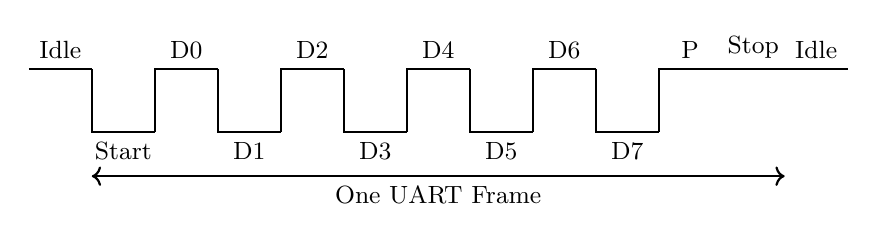
\begin{tikzpicture}[scale=0.8]
  % Idle state
  \draw[thick] (0,1) -- (1,1) node[midway,above] {\small Idle};
  
  % Start bit
  \draw[thick] (1,1) -- (1,0) -- (2,0) node[midway,below] {\small Start};
  
  % Data bits
  \draw[thick] (2,0) -- (2,1) -- (3,1) node[midway,above] {\small D0};
  \draw[thick] (3,1) -- (3,0) -- (4,0) node[midway,below] {\small D1};
  \draw[thick] (4,0) -- (4,1) -- (5,1) node[midway,above] {\small D2};
  \draw[thick] (5,1) -- (5,0) -- (6,0) node[midway,below] {\small D3};
  \draw[thick] (6,0) -- (6,1) -- (7,1) node[midway,above] {\small D4};
  \draw[thick] (7,1) -- (7,0) -- (8,0) node[midway,below] {\small D5};
  \draw[thick] (8,0) -- (8,1) -- (9,1) node[midway,above] {\small D6};
  \draw[thick] (9,1) -- (9,0) -- (10,0) node[midway,below] {\small D7};
  
  % Parity bit
  \draw[thick] (10,0) -- (10,1) -- (11,1) node[midway,above] {\small P};
  
  % Stop bit
  \draw[thick] (11,1) -- (12,1) node[midway,above] {\small Stop};
  
  % Idle again
  \draw[thick] (12,1) -- (13,1) node[midway,above] {\small Idle};
  
  % Labels
  \draw[<->,thick] (1,-0.7) -- (12,-0.7);
  \node at (6.5,-1) {\small One UART Frame};
\end{tikzpicture}
\caption{UART Frame Structure (8 data bits, 1 parity bit, 1 stop bit)}
\end{figure}

\noindent
\textbf{Common UART Configuration: 8N1}
\begin{itemize}[nosep]
  \item 8 data bits
  \item No parity (N)
  \item 1 stop bit
  \item Most widely used configuration for simplicity and efficiency
\end{itemize}

\subsubsection{Baud Rate}

The \textbf{baud rate} is the rate at which symbols (bits) are transmitted per second, measured in bits per second (bps). Common baud rates include:

\begin{itemize}[nosep]
  \item \textbf{9600 bps}: Slow, highly reliable, long cable lengths
  \item \textbf{115200 bps}: Fast, common for debugging and short cables
  \item \textbf{Other rates}: 4800, 19200, 38400, 57600, 230400, 460800, 921600 bps
\end{itemize}

\noindent
Both transmitter and receiver must use the \textit{exact same} baud rate. Even small differences (> 2-3\%) can cause communication errors due to timing drift over the duration of a frame.

\subsubsection{Full-Duplex Communication}

UART supports \textbf{full-duplex} communication, meaning data can be transmitted and received simultaneously on separate lines:
\begin{itemize}[nosep]
  \item \textbf{TX (Transmit)}: Output pin for sending data
  \item \textbf{RX (Receive)}: Input pin for receiving data
  \item \textbf{Connection}: TX of device A connects to RX of device B, and vice versa
  \item \textbf{Ground}: Shared ground reference is essential for proper voltage level detection
\end{itemize}

\subsection{TM4C123 UART Architecture}

The TM4C123 microcontroller includes eight UART modules (UART0-UART7) with advanced features:

\subsubsection{UART Features}
\begin{itemize}[nosep]
  \item \textbf{Baud rate generation}: Programmable from 300 bps to 5 Mbps
  \item \textbf{Data formats}: 5, 6, 7, 8, or 9 data bits
  \item \textbf{Parity}: Even, odd, or no parity
  \item \textbf{Stop bits}: 1 or 2 stop bits
  \item \textbf{FIFOs}: 16-byte transmit and receive FIFOs with programmable trigger levels
  \item \textbf{Interrupts}: Transmit, receive, overrun, framing error, parity error, break detection
  \item \textbf{DMA support}: Direct Memory Access for high-throughput transfers
  \item \textbf{IrDA and 9-bit modes}: Advanced communication modes
\end{itemize}

\subsubsection{UART Pin Mapping}

Each UART module is mapped to specific GPIO pins through alternate function configuration:

\begin{table}[H]
\centering
\small
\renewcommand{\arraystretch}{1.2}
\begin{tabular}{llll}
\toprule
\textbf{UART Module} & \textbf{TX Pin} & \textbf{RX Pin} & \textbf{Notes} \\
\midrule
UART0 & PA1 & PA0 & Connected to USB-to-serial on LaunchPad \\
UART1 & PB1 & PB0 & Available on expansion headers \\
UART2 & PD7 & PD6 & Available on expansion headers \\
UART3 & PC7 & PC6 & Available on expansion headers \\
UART4 & PC5 & PC4 & Available on expansion headers \\
UART5 & PE5 & PE4 & Available on expansion headers \\
UART6 & PD5 & PD4 & Available on expansion headers \\
UART7 & PE1 & PE0 & Available on expansion headers \\
\bottomrule
\end{tabular}
\caption{TM4C123 UART Pin Assignments}
\end{table}

\noindent
In this experiment, we use \textbf{UART0} (PA0/PA1) because it is directly connected to the on-board USB-to-serial converter, allowing easy communication with a PC terminal without additional hardware.

\subsection{UART Registers}

The UART modules are controlled through memory-mapped registers. Key registers include:

\subsubsection{UARTDR — Data Register}
\noindent\textbf{Register:} \texttt{UARTx->DR} — UART Data (\texttt{Base + 0x000})

\noindent
The Data Register is used for both transmitting and receiving data:
\begin{itemize}[nosep]
  \item \textbf{Write}: Places data in the transmit FIFO (bits 7:0 contain the byte to transmit)
  \item \textbf{Read}: Retrieves data from the receive FIFO (bits 7:0 contain the received byte)
  \item \textbf{Error flags} (bits 11:8 on read): Framing Error (FE), Parity Error (PE), Break Error (BE), Overrun Error (OE)
\end{itemize}

\subsubsection{UARTFR — Flag Register}
\noindent\textbf{Register:} \texttt{UARTx->FR} — UART Flag Register (\texttt{Base + 0x018})

\noindent
The Flag Register provides status information about the UART:

\begin{table}[H]
\centering
\small
\renewcommand{\arraystretch}{1.2}
\begin{tabular}{clp{7cm}}
\toprule
\textbf{Bit} & \textbf{Name} & \textbf{Description} \\
\midrule
0 & CTS & Clear To Send (hardware flow control, not commonly used) \\
3 & BUSY & UART busy transmitting data \\
4 & RXFE & Receive FIFO Empty (1 = empty, 0 = data available) \\
5 & TXFF & Transmit FIFO Full (1 = full, wait before writing) \\
6 & RXFF & Receive FIFO Full \\
7 & TXFE & Transmit FIFO Empty (1 = empty, transmission complete) \\
\bottomrule
\end{tabular}
\caption{UARTFR Register Bits}
\end{table}

\subsubsection{UARTIBRD and UARTFBRD — Baud Rate Divisors}
\noindent\textbf{Registers:} \texttt{UARTx->IBRD} and \texttt{UARTx->FBRD}

\noindent
The baud rate is determined by dividing the UART clock by a divisor:

\[
\text{Baud Rate} = \frac{f_{\text{UART clock}}}{16 \times (\text{IBRD} + \text{FBRD})}
\]

\noindent
Where:
\begin{itemize}[nosep]
  \item \textbf{IBRD}: Integer part of the baud rate divisor (16-bit value)
  \item \textbf{FBRD}: Fractional part of the baud rate divisor (6-bit value, represents fraction/64)
\end{itemize}

\noindent
\textbf{Calculation Steps:}
\begin{enumerate}[nosep]
  \item Calculate divisor: $\text{Divisor} = \frac{f_{\text{UART clock}}}{16 \times \text{Baud Rate}}$
  \item Integer part: $\text{IBRD} = \lfloor \text{Divisor} \rfloor$
  \item Fractional part: $\text{FBRD} = \text{round}((\text{Divisor} - \text{IBRD}) \times 64 + 0.5)$
\end{enumerate}

\noindent
\textbf{Example: 115200 baud at 50 MHz system clock}
\[
\text{Divisor} = \frac{50{,}000{,}000}{16 \times 115{,}200} = \frac{50{,}000{,}000}{1{,}843{,}200} \approx 27.126
\]
\[
\text{IBRD} = 27, \quad \text{FBRD} = \text{round}(0.126 \times 64 + 0.5) = \text{round}(8.564) = 8
\]

\subsubsection{UARTLCRH — Line Control Register}
\noindent\textbf{Register:} \texttt{UARTx->LCRH} — UART Line Control (\texttt{Base + 0x02C})

\noindent
The Line Control Register configures the frame format:

\begin{table}[H]
\centering
\small
\renewcommand{\arraystretch}{1.2}
\begin{tabular}{clp{6.5cm}}
\toprule
\textbf{Bits} & \textbf{Name} & \textbf{Description} \\
\midrule
0 & BRK & Send break (force TX low) \\
1 & PEN & Parity Enable (0 = no parity, 1 = parity enabled) \\
2 & EPS & Even Parity Select (0 = odd, 1 = even) \\
3 & STP2 & Two Stop Bits (0 = 1 stop bit, 1 = 2 stop bits) \\
4 & FEN & FIFO Enable (0 = disable FIFOs, 1 = enable FIFOs) \\
6:5 & WLEN & Word Length: 00 = 5 bits, 01 = 6 bits, 10 = 7 bits, 11 = 8 bits \\
7 & SPS & Stick Parity Select \\
\bottomrule
\end{tabular}
\caption{UARTLCRH Register Bits}
\end{table}

\noindent
\textbf{Common configuration (8N1 with FIFOs):}
\begin{lstlisting}[language=C]
UART0->LCRH = (0x3 << 5) | (1 << 4);  // 8 data bits, FIFOs enabled
// Or: UART0->LCRH = 0x60;
\end{lstlisting}

\subsubsection{UARTCTL — Control Register}
\noindent\textbf{Register:} \texttt{UARTx->CTL} — UART Control (\texttt{Base + 0x030})

\noindent
The Control Register enables/disables the UART and its transmit/receive functions:

\begin{table}[H]
\centering
\small
\renewcommand{\arraystretch}{1.2}
\begin{tabular}{clp{7cm}}
\toprule
\textbf{Bit} & \textbf{Name} & \textbf{Description} \\
\midrule
0 & UARTEN & UART Enable (0 = disable, 1 = enable) \\
8 & TXE & Transmit Enable (0 = disable TX, 1 = enable TX) \\
9 & RXE & Receive Enable (0 = disable RX, 1 = enable RX) \\
\bottomrule
\end{tabular}
\caption{UARTCTL Register Key Bits}
\end{table}

\noindent
\textbf{Enable UART with TX and RX:}
\begin{lstlisting}[language=C]
UART0->CTL = (1 << 0) | (1 << 8) | (1 << 9);  // Enable UART, TX, RX
// Or: UART0->CTL = 0x301;
\end{lstlisting}

\subsubsection{UARTCC — Clock Configuration}
\noindent\textbf{Register:} \texttt{UARTx->CC} — UART Clock Configuration (\texttt{Base + 0xFC8})

\noindent
Selects the clock source for the UART module:
\begin{itemize}[nosep]
  \item \texttt{0x0}: System clock (default and most common)
  \item \texttt{0x5}: PIOSC (16 MHz internal oscillator)
\end{itemize}

\subsection{UART Configuration Workflow}

The following steps configure UART0 for basic serial communication:

\begin{enumerate}[nosep]
  \item \textbf{Enable clocks}: Enable UART0 and GPIOA clocks in \texttt{SYSCTL->RCGCUART} and \texttt{SYSCTL->RCGCGPIO}
  \item \textbf{Wait for clock stabilization}: Check ready bits or insert delay
  \item \textbf{Disable UART}: Clear \texttt{UART0->CTL} during configuration
  \item \textbf{Configure GPIO for UART alternate function}:
    \begin{itemize}[nosep]
      \item Enable alternate function: \texttt{GPIOA->AFSEL |= 0x03} (PA0, PA1)
      \item Set port control: \texttt{GPIOA->PCTL |= 0x11} (UART function on PA0/PA1)
      \item Enable digital: \texttt{GPIOA->DEN |= 0x03}
    \end{itemize}
  \item \textbf{Set baud rate divisors}: Write \texttt{UART0->IBRD} and \texttt{UART0->FBRD}
  \item \textbf{Configure line control}: Set data bits, parity, stop bits, enable FIFOs in \texttt{UART0->LCRH}
  \item \textbf{Select clock source}: \texttt{UART0->CC = 0} (system clock)
  \item \textbf{Enable UART}: Set \texttt{UART0->CTL} to enable UART, TX, and RX
\end{enumerate}

\newpage
\section{Procedure}

\subsection{Example: Basic UART Driver Implementation}

The following code demonstrates a complete UART driver for UART0 with initialization, character/string transmission, and character/string reception.

\subsubsection{UART Header File}

\lstinputlisting[language=C, caption={UART driver header file (\texttt{uart.h})}]{snippets/uart/uart.h}

\subsubsection{UART Implementation File}

\lstinputlisting[language=C, caption={UART driver implementation (\texttt{uart.c})}]{snippets/uart/uart.c}

\subsubsection{Main Application}

\lstinputlisting[language=C, caption={Main application using UART driver (\texttt{main.c})}]{snippets/uart/main.c}

\subsection{Code Explanation}

\paragraph{UART Initialization}
The \texttt{UART0\_Init()} function configures UART0 for 115200 baud, 8N1 format with FIFOs enabled:
\begin{enumerate}[nosep]
  \item Enables UART0 and GPIOA clocks
  \item Configures PA0 (RX) and PA1 (TX) for UART alternate function using AFSEL, PCTL, and DEN
  \item Disables UART0 during configuration
  \item Sets baud rate divisors: IBRD = 27, FBRD = 8 for 115200 baud at 50 MHz
  \item Configures line control: 8 data bits (\texttt{WLEN = 0x3}), FIFOs enabled (\texttt{FEN = 1})
  \item Selects system clock as UART clock source
  \item Enables UART0 with transmit and receive functions
\end{enumerate}

\paragraph{Transmitting Data}
The \texttt{UART0\_WriteChar()} function sends a single character:
\begin{itemize}[nosep]
  \item Polls the TXFF flag (bit 5) in the FR register
  \item Waits while TXFF = 1 (transmit FIFO full)
  \item Writes character to DR register when FIFO has space
  \item Hardware automatically handles framing (start bit, data bits, stop bit)
\end{itemize}

\noindent
The \texttt{UART0\_WriteString()} function sends a null-terminated string by repeatedly calling \texttt{UART0\_WriteChar()}.

\paragraph{Receiving Data}
The \texttt{UART0\_ReadChar()} function receives a single character:
\begin{itemize}[nosep]
  \item Polls the RXFE flag (bit 4) in the FR register
  \item Waits while RXFE = 1 (receive FIFO empty)
  \item Reads character from DR register when data is available
  \item Masks to 8 bits (\texttt{0xFF}) to extract data byte
\end{itemize}

\noindent
The \texttt{UART0\_ReadString()} function reads characters until Enter (\texttt{\textbackslash r} or \texttt{\textbackslash n}), with optional echo.

\paragraph{Main Application}
The main program demonstrates:
\begin{enumerate}[nosep]
  \item UART initialization
  \item Sending a greeting message
  \item Echo loop: reading a string, echoing it back with a prefix
\end{enumerate}

\subsection{Using PuTTY for Serial Communication}

To interact with the TM4C123 via UART0, use a terminal emulator like PuTTY:

\begin{enumerate}[nosep]
  \item Download and install PuTTY from \url{https://www.putty.org/}
  \item Connect the TM4C123 LaunchPad to your PC via USB
  \item Open Windows Device Manager and find the COM port under ``Ports (COM \& LPT)'' (e.g., COM3)
  \item Launch PuTTY and configure:
    \begin{itemize}[nosep]
      \item Connection type: Serial
      \item Serial line: COMx (replace with your COM port)
      \item Speed: 115200 (or your configured baud rate)
    \end{itemize}
  \item Click ``Open'' to establish connection
  \item Type text and press Enter to send strings to the microcontroller
  \item View echoed responses and debug output
\end{enumerate}

\begin{figure}[H]
\centering
\includegraphics[width=0.6\textwidth]{resources/putty.png}
\caption{PuTTY Serial Configuration}
\label{fig:putty_config}
\end{figure}

\noindent
\textbf{Tip}: Enable ``Local echo'' in PuTTY settings (Terminal → Line discipline options) to see your typed characters even before the microcontroller echoes them back.

\newpage
\subsection{Tasks}

\subsubsection{Task 1: LED Control via UART Commands}

Write a program that receives single-character commands via UART to control the on-board LEDs.

\paragraph{Requirements:}
\begin{itemize}[nosep]
  \item Initialize UART0 and configure GPIO Port F for LEDs (PF1/Red, PF2/Blue, PF3/Green)
  \item Receive single characters via UART0
  \item Implement command processing:
    \begin{itemize}[nosep]
      \item \texttt{'r'} or \texttt{'R'}: Toggle RED LED
      \item \texttt{'b'} or \texttt{'B'}: Toggle BLUE LED
      \item \texttt{'g'} or \texttt{'G'}: Toggle GREEN LED
      \item \texttt{'a'} or \texttt{'A'}: Turn all LEDs ON
      \item \texttt{'x'} or \texttt{'X'}: Turn all LEDs OFF
    \end{itemize}
  \item Echo back confirmation messages (e.g., ``RED LED toggled'')
  \item Send error message for unrecognized commands
\end{itemize}

\paragraph{Hint:}
\begin{lstlisting}[language=C]
char cmd = UART0_ReadChar();
switch (cmd) {
    case 'r':
    case 'R':
        GPIOF->DATA ^= (1 << 1);  // Toggle RED
        UART0_WriteString("RED LED toggled\r\n");
        break;
    // ... other cases
    default:
        UART0_WriteString("Unknown command\r\n");
}
\end{lstlisting}

\subsubsection{Task 2: ADC Value Monitoring}

Create a program that reads the on-board temperature sensor (or potentiometer) using ADC and continuously sends the values to a PC terminal.

\paragraph{Requirements:}
\begin{itemize}[nosep]
  \item Initialize UART0 for serial communication
  \item Initialize ADC0 to read the internal temperature sensor (ADC0 sequencer 3)
  \item Use a timer (SysTick or GPTM) to trigger ADC sampling every 1 second
  \item Convert ADC value to temperature in degrees Celsius using the formula:
    \[
    T_{\text{C}} = 147.5 - \frac{(\text{ADC\_Value} \times 3.3 \times 100)}{4096}
    \]
  \item Format and send the temperature reading via UART (e.g., ``Temp: 25.3 C'')
  \item Use \texttt{sprintf()} to format floating-point values into strings
\end{itemize}

\paragraph{Hint:}
\begin{lstlisting}[language=C]
#include <stdio.h>

char buffer[50];
float temp = 147.5 - ((adcValue * 3.3 * 100) / 4096.0);
sprintf(buffer, "Temperature: %.1f C\r\n", temp);
UART0_WriteString(buffer);
\end{lstlisting}

\subsubsection{Task 3: Simple Command-Line Interface}

Implement a simple command-line interface (CLI) that accepts multi-character commands and arguments.

\paragraph{Requirements:}
\begin{itemize}[nosep]
  \item Display a welcome message and prompt (``>'') after initialization
  \item Read complete strings (terminated by Enter) using \texttt{UART0\_ReadString()}
  \item Parse commands with arguments (e.g., ``LED RED ON'', ``DELAY 500'')
  \item Implement command processing:
    \begin{itemize}[nosep]
      \item \texttt{LED <color> <ON|OFF>}: Control specific LED
      \item \texttt{BLINK <color> <count>}: Blink LED specified number of times
      \item \texttt{STATUS}: Report current LED states
      \item \texttt{HELP}: Display available commands
    \end{itemize}
  \item Send confirmation or error messages
  \item Display prompt after each command execution
\end{itemize}

\paragraph{Hint:}
Use \texttt{strcmp()} and \texttt{strtok()} for string parsing:
\begin{lstlisting}[language=C]
#include <string.h>

char buffer[50];
UART0_ReadString(buffer, 50);

char *cmd = strtok(buffer, " ");
if (strcmp(cmd, "LED") == 0) {
    char *color = strtok(NULL, " ");
    char *state = strtok(NULL, " ");
    // Process LED command
} else if (strcmp(cmd, "STATUS") == 0) {
    // Report status
}
UART0_WriteString("> ");  // Display prompt
\end{lstlisting}

\subsection{Testing and Debugging}

\subsubsection{Common Issues and Solutions}

\paragraph{No output in terminal}
\begin{itemize}[nosep]
  \item \textbf{Cause}: Wrong COM port, incorrect baud rate, or UART not initialized
  \item \textbf{Solution}: Verify COM port in Device Manager, ensure baud rates match (115200), check UART initialization code
\end{itemize}

\paragraph{Garbled characters}
\begin{itemize}[nosep]
  \item \textbf{Cause}: Baud rate mismatch between microcontroller and terminal
  \item \textbf{Solution}: Recalculate IBRD and FBRD values, verify system clock frequency, ensure terminal baud rate matches code
\end{itemize}

\paragraph{Missing characters or corrupted data}
\begin{itemize}[nosep]
  \item \textbf{Cause}: FIFO overrun, insufficient processing speed, timing issues
  \item \textbf{Solution}: Enable FIFOs, process received data promptly, consider interrupt-driven reception for high data rates
\end{itemize}

\paragraph{Characters not echoing back}
\begin{itemize}[nosep]
  \item \textbf{Cause}: RX not configured, GPIO alternate function not set correctly
  \item \textbf{Solution}: Verify GPIOA->AFSEL, GPIOA->PCTL, GPIOA->DEN settings, ensure RXE bit is set in UART0->CTL
\end{itemize}

\subsubsection{Debugging Strategy}

\begin{enumerate}[nosep]
  \item \textbf{Test transmission first}: Send fixed strings to verify TX is working before implementing RX
  \item \textbf{Use LED indicators}: Toggle LEDs after UART initialization and during character transmission/reception
  \item \textbf{Verify clock configuration}: Ensure system clock is 50 MHz as expected
  \item \textbf{Check register values}: Use debugger to inspect UART registers (CTL, FR, IBRD, FBRD, LCRH)
  \item \textbf{Test with simple echo}: Start with single-character echo before implementing complex string processing
  \item \textbf{Monitor FIFO flags}: Check TXFF and RXFE flags to ensure proper FIFO operation
\end{enumerate}

\subsubsection{Advanced UART Features}

For more sophisticated applications, consider exploring:
\begin{itemize}[nosep]
  \item \textbf{Interrupt-driven I/O}: Use UART interrupts instead of polling for better CPU efficiency
  \item \textbf{DMA transfers}: Offload large data transfers to DMA controller
  \item \textbf{Hardware flow control}: Implement RTS/CTS for reliable high-speed communication
  \item \textbf{9-bit mode}: Support address/data distinction in multi-processor systems
  \item \textbf{LIN and IrDA modes}: Special communication protocols for automotive and infrared applications
\end{itemize}


\clearpage
\ifodd\value{page}
  % already odd: do nothing 
\else
  \thispagestyle{empty}\null\newpage
\fi
\end{document}

